\documentclass[11pt, a4paper]{report}
\usepackage{vntex}
%\usepackage[english,vietnam]{babel}
%\usepackage[utf8]{inputenc}
%\usepackage{mathptmx}[ptm]
%\usepackage[utf8]{inputenc}
%\usepackage[francais]{babel}
\usepackage{a4wide,amssymb,epsfig,latexsym,array,hhline,fancyhdr}
\usepackage[normalem]{ulem}
%\usepackage{soul}

\usepackage[makeroom]{cancel}
\usepackage{amsmath}
\usepackage{amsthm}
\usepackage{multicol,longtable,amscd}
\usepackage{diagbox}%Make diagonal lines in tables
\usepackage{booktabs}
\usepackage{alltt}
\usepackage[framemethod=tikz]{mdframed}% For highlighting paragraph backgrounds
\usepackage{caption,subcaption}

\usepackage{lastpage}
\usepackage[lined,boxed,commentsnumbered]{algorithm2e}
\usepackage{enumerate}
\usepackage{color}
\usepackage{graphicx}							% Standard graphics package
\usepackage{array}
\usepackage{tabularx, caption}
\usepackage{multirow}
\usepackage{multicol}
\usepackage{rotating}
\usepackage{graphics}
\usepackage{geometry}
\usepackage{setspace}
\usepackage{epsfig}
\usepackage{tikz}
\usepackage{titlesec}


\usetikzlibrary{arrows,snakes,backgrounds,calc}
\usepackage[unicode]{hyperref}
\hypersetup{urlcolor=blue,linkcolor=black,citecolor=black,colorlinks=true} 
\usepackage{listings}

%\usepackage{pstcol} 								% PSTricks with the standard color package

\usepackage[normalem]{ulem}

\usepackage{titlesec}
\setcounter{secnumdepth}{4}
\renewcommand{\theparagraph}{\Alph{paragraph}}
\titleformat{\paragraph}
{\normalfont\normalsize\bfseries}{\theparagraph}{1em}{} 
\titlespacing*{\paragraph}
{0pt}{3.25ex plus 1ex minus .2ex}{1.5ex plus .2ex}

\setcounter{secnumdepth}{4}
\renewcommand{\theparagraph}{\Alph{paragraph}}
\titleformat{\paragraph}
{\normalfont\normalsize\bfseries}{\theparagraph}{1em}{} 
\titlespacing*{\paragraph}
{0pt}{3.25ex plus 1ex minus .2ex}{1.5ex plus .2ex}
\newtheorem{theorem}{{\bf Định lý}}
\newtheorem{property}{{\bf Tính chất}}
\newtheorem{proposition}{{\bf Mệnh đề}}
\newtheorem{corollary}[proposition]{{\bf Hệ quả}}
\newtheorem{lemma}[proposition]{{\bf Bổ đề}}
\theoremstyle{definition}
\newtheorem{exer}{Bài toán}
\addtocontents{toc}{\protect\thispagestyle{empty}}
% Remove page number in contents page. 
\addtocontents{lof}{\protect\thispagestyle{empty}}
% Remove page number in list of figure page. 
\addtocontents{lot}{\protect\thispagestyle{empty}}
% Remove page number in list of table page. 
\def\thesislayout{	% A4: 210 × 297
	\geometry{
		a4paper,
		total={160mm,240mm},  % fix over page
		left=30mm,
		top=22mm,
            right=20mm,
            bottom=20mm,
	}
}
\def\thesisheadlayout{	% A4: 210 × 297
	\geometry{
		a4paper,
		total={160mm,240mm},  % fix over page
		left=30mm,
		top=10mm,
	}
}
\thesislayout
\lstset{
language=R,
basicstyle=\footnotesize\sffamily,
commentstyle=\ttfamily\color{black},
numbers=left,
numberstyle=\ttfamily\color{black}\footnotesize,
stepnumber=1,
numbersep=5pt,
backgroundcolor=\color{white},
showspaces=false,
showstringspaces=false,
showtabs=false,
frame=single,
tabsize=2,
captionpos=b,
breaklines=true,
breakatwhitespace=false,
title=\lstname,
escapeinside={},
keywordstyle={},
morekeywords={}
}
%\usepackage{fancyhdr}
\renewcommand{\baselinestretch}{1.3}
\setlength{\headheight}{40pt}
\pagestyle{fancy}
\fancyhead{} % clear all header fields
\renewcommand{\footruleskip}{1mm}

\fancyhead[L]{
 \begin{tabular}{rl}
    \begin{picture}(25,15)(0,0)
    \put(0,-8){
\includegraphics[width=10mm, height=10mm]{Images/hcmut.png}}
    %\put(0,-8){\epsfig{width=10mm,figure=hcmut.eps}}
   \end{picture}&
	%\includegraphics[width=8mm, height=8mm]{hcmut.png} & %
	\begin{tabular}{l}
		\textbf{  Trường Đại Học Bách Khoa - Đại học Quốc gia TP.HCM }\\
		\textbf{  Khoa Khoa Học \& Kỹ Thuật Máy Tính}
	\end{tabular} 	
 \end{tabular}
}
\fancyhead[R]{
	\begin{tabular}{l}
		\tiny \bf \\
		\tiny \bf 
	\end{tabular}  }
\fancyfoot{} % clear all footer fields
\fancyfoot[L]{\scriptsize  Đồ án môn học Kỹ thuật Máy tính - CO4041}
\fancyfoot[R]{\scriptsize  Trang {\thepage}/\pageref{LastPage}}

\renewcommand{\headrulewidth}{0.3pt}
\renewcommand{\footrulewidth}{0.3pt}

%%%
\setcounter{secnumdepth}{4}
\setcounter{tocdepth}{3}
\makeatletter
\newcounter {subsubsubsection}[subsubsection]
\renewcommand\thesubsubsubsection{\thesubsubsection .\@alph\c@subsubsubsection}
\newcommand\subsubsubsection{\@startsection{subsubsubsection}{4}{\z@}%
                                     {-3.25ex\@plus -1ex \@minus -.2ex}%
                                     {1.5ex \@plus .2ex}%
                                     {\normalfont\normalsize\bfseries}}
\newcommand*\l@subsubsubsection{\@dottedtocline{3}{10.0em}{4.1em}}
\newcommand*{\subsubsubsectionmark}[1]{}
\makeatother

\everymath{\color{black}}%make in-line maths symbols blue to read/check easily

\sloppy
\captionsetup[figure]{labelfont={small,bf},textfont={small,it},belowskip=-1pt,aboveskip=-9pt}
%space remove between caption, figure, and text
\captionsetup[table]{labelfont={small,bf},textfont={small,it},belowskip=-1pt,aboveskip=7pt}
\setlength{\floatsep}{5pt plus 2pt minus 2pt}
\setlength{\textfloatsep}{5pt plus 2pt minus 2pt}
\setlength{\intextsep}{10pt plus 2pt minus 2pt}

\thesislayout

\begin{document}

\begin{titlepage}
\begin{tikzpicture}[remember picture, overlay]
  \draw[line width = 4pt] ($(current page.north west) + (0.4in,-0.5in)$) rectangle ($(current page.south east) + (-0.4in,0.5in)$);
  \draw[line width=1.5pt]
    ($ (current page.north west) + (0.45in,-0.55in) $)
    rectangle
    ($ (current page.south east) + (-0.45in,0.55in) $);
\end{tikzpicture}

\begin{center}
\Large \textbf{ĐẠI HỌC QUỐC GIA THÀNH PHỐ HỒ CHÍ MINH} \\
\Large \textbf{TRƯỜNG ĐẠI HỌC BÁCH KHOA} \\
\Large \textbf{KHOA KHOA HỌC VÀ KĨ THUẬT MÁY TÍNH}
\end{center}


\begin{figure}[h!]
\begin{center}

\includegraphics[width=4cm]{Images/hcmut.png}
\end{center}
\end{figure}

\begin{center}
\begin{tabular}{c}
\multicolumn{1}{c}{\textbf{{\LARGE BÁO CÁO}}}\\
\\{\textbf{{\LARGE ĐỒ ÁN MÔN HỌC KỸ THUẬT MÁY TÍNH}}}
\\
\textbf{\LARGE Hiện thực bộ tăng tốc CNN dựa trên RISC-V}
\\
%\textbf{\LARGE CNN dựa trên RISC-V}
%\\

{\Large NGÀNH: KỸ THUẬT MÁY TÍNH}
\end{tabular}
\end{center}
\begin{table}[h]
\begin{tabular}{rll}
\hspace{5 cm} &  \textbf{\Large HỘI ĐỒNG:} {}
\\
\vspace{2cm}
\\
% & \hspace{3.2cm} \Large{PGS.TS Trần Ngọc Thịnh}
% \\
% \\
% & \hspace{3.2cm} \Large{PGS.TS Phạm Quốc Cường}
% \\
% \\
% & \hspace{3.2cm} \Large{Huỳnh Phúc Nghị}
% \\
% \\
\hspace{5cm} &   \textbf{\Large GVHD:} \hspace{1.3cm}{\Large Th.S Huỳnh Phúc Nghị}
\\
\\
& \hspace{3.23cm} \Large{PGS.TS Trần Ngọc Thịnh}
\\
\\
% \hspace{5 cm}  &   \textbf{\Large TKHĐ:} \hspace{1.35cm}{\Large Huỳnh Phúc Nghị}
% \\
% \\
% TKHĐ là THƯ KÝ HỘI ĐỒNG
\hspace{4 cm} &     \textbf{$\;$ $\;$$\;$$\;$$\;$$\;$$\;$$\;$$\;$$\;$$\;$$\;$$\;$$\;$$\;$$\;$$\;$$\;$$\;$$\;$$\;$$\;$$\;$$\;$$\;$$\;$$\;$$\;$$\;$$\;$$\;$$\;$$\;$$\;$ \Large ---o0o---} 
\\
\\
\hspace{4 cm} &   \textbf{\Large SVTH:} \hspace{1.5cm}{\Large Nguyễn Văn Nam - 2114121}
\\
\\
\\
\\
\end{tabular}
\end{table}
\vspace{0.5cm}
\begin{center}
{\Large TP. HỒ CHÍ MINH, THÁNG 12/2025 }
\end{center}
\end{titlepage}
%\thispagestyle{empty}
\newpage
% \chapter*{Chữ ký của GVHD}

\vspace{2cm} % Vertical spacing

% Supervisor 1
\noindent
\begin{tabular}{p{8cm}p{4cm}}
\hrulefill & Ngày: \hrulefill \\
PGS. TS. Trần Ngọc Thịnh \\ 
\textit{Phó Giáo sư} & \\
\textit{Khoa Khoa học và Kỹ thuật Máy tính} & \\
\end{tabular}

\vspace{3cm} % Spacing between entries

% Supervisor 2
\noindent
\begin{tabular}{p{8cm}p{4cm}}
\hrulefill & Ngày: \hrulefill \\
Huỳnh Phúc Nghị \\
\textit{Khoa Khoa học và Kỹ thuật Máy tính} & \\
\end{tabular}

% \newpage
%%%%%%%%%%%%%%%%%INTRO%%%%%%%%%%%%%%%%%%%
\chapter*{Lời cam đoan}
% Manual confirmation required before submission. Reference wording exists in
% RISC_V_AIoT_Capstone_Project_Print_V1.pdf, PDF page 2, but is another
% student's declaration, not a verified current institutional form. Confirm the
% required wording, acknowledgements of reused work, date and signature.
\noindent\textit{[Chờ xác nhận nội dung lời cam đoan theo mẫu áp dụng.]}
\vfill
\begin{flushright}
\textit{[Địa điểm, ngày tháng năm]}\\[1em]
Người thực hiện\\[3em]
Nguyễn Văn Nam
\end{flushright}

\newpage
\chapter*{Lời cảm ơn}
$\indent$Trong suốt quá trình học tập  em luôn được sự quan tâm, hướng dẫn và giúp đỡ tận tình của các thầy, cô giáo trong Khoa Khoa học \& Kỹ thuật Máy tính cùng với sự động viên giúp đỡ của bạn bè.\\
\\
$\indent$Em cũng xin chân thành cảm ơn các thầy cô giáo trong trường Đại học Bách Khoa - Đại học Quốc gia Thành phố Hồ Chí Minh nói chung, các thầy cô trong Khoa Khoa học \& Kỹ thuật Máy tính nói riêng đã dạy dỗ cho em kiến thức về các môn đại cương cũng như các môn chuyên ngành, giúp em có được cơ sở lý thuyết vững vàng và tạo điều kiện giúp đỡ em trong suốt quá trình học tập.\\
\\
$\indent$Đặc biệt, em xin bày tỏ sự kính trọng và lòng biết ơn sâu sắc nhất đến Th.S Huỳnh Phúc Nghị và PGS. TS. Trần Ngọc Thịnh, hai thầy là người đã trực tiếp hướng dẫn, giúp đỡ cho em để em có thể hoàn thành đồ án này. Trong quá trình học tập và nghiên cứu, nếu em có những sai sót gì, kính mong thầy cô bỏ qua cho em!\\
\\
$\indent$Cuối cùng, em xin chân thành cảm ơn gia đình và bạn bè, đã luôn tạo điều kiện, quan tâm, giúp đỡ, động viên em trong suốt quá trình học tập và hoàn thành đồ án này.\\
\\
$\indent$Với điều kiện thời gian cũng như kinh nghiệm còn hạn chế của một học viên, đồ án này không thể tránh được những thiếu sót. Em rất mong nhận được sự chỉ bảo, đóng góp ý kiến của các thầy cô để tôi có điều kiện bổ sung, nâng cao ý thức của mình, phục vụ tốt hơn công tác thực tế sau này.\\
\\
$\indent$Em xin trân trọng cảm ơn!
\newpage
% \chapter*{Tóm tắt nội dung}

\newpage
\tableofcontents
\newpage
\listoffigures
\newpage
%\listoftables
\newpage
\setcounter{page}{1}

%%%%%%%%%%%%%%%%%CONTENTS%%%%%%%%%%%%%%%%%%%
\chapter{GIỚI THIỆU ĐỀ TÀI}
\label{chap:gioithieu}

\section{Động cơ thực hiện đề tài}
Suy luận mạng nơ-ron tại thiết bị biên cho phép xử lý dữ liệu gần nơi phát sinh. Tuy nhiên, các hệ thống nhúng thường bị giới hạn về năng lực tính toán và dung lượng bộ nhớ. Với mạng nơ-ron tích chập (Convolutional Neural Network, CNN), số lượng phép nhân--cộng và các lần truy cập tensor có thể làm thời gian suy luận trên một CPU nhỏ trở nên lớn. Hiệu quả năng lượng là một động cơ chung của tính toán tại biên; trong đề tài này, các đại lượng được đánh giá là tính đúng đắn, số chu kỳ, tài nguyên FPGA và timing.

Phần cứng chuyên dụng có thể giảm chi phí thực hiện một số phép toán CNN, nhưng cần thêm tài nguyên lưu trữ, datapath và logic điều khiển. Khi CPU phải cấp toán hạng và thu kết quả qua các thanh ghi ánh xạ bộ nhớ, chi phí truyền dữ liệu có thể hạn chế lợi ích của datapath. Vì vậy, lựa chọn phần việc đưa xuống phần cứng phải gắn với cách firmware tổ chức dữ liệu và gọi bộ tăng tốc.

Từ vấn đề đó, đề tài hiện thực MyTinyMobileNetSoC, một hệ thống dựa trên PicoRV32 để suy luận TinyMobileNet trên dữ liệu MNIST. Workload có các lớp tích chập chuẩn, depthwise và pointwise, cho phép khảo sát những yêu cầu khác nhau về tính toán và tái sử dụng dữ liệu trong cùng một đường suy luận. Trọng tâm là xây dựng hệ thống hoạt động tích hợp, xác định nút thắt bằng số đo và cải thiện hiệu năng qua đồng thiết kế phần cứng--phần mềm (HW/SW co-design).

\section{Bài toán đặt ra}
Tăng tốc CNN không chỉ là tăng tốc số học. Trong MyTinyMobileNetSoC, CPU đọc tensor từ RAM, ghi toán hạng qua MMIO, điều khiển thực thi và đọc kết quả về. CPU còn điều phối thứ tự lớp, cộng bias, xử lý offset và giới hạn giá trị đầu ra. Các bộ tăng tốc không tự truy cập RAM và không có giao diện DMA.

Do đó, hiệu năng phụ thuộc đồng thời vào điều khiển CPU, số giao dịch MMIO, khả năng tái sử dụng dữ liệu, lịch vòng lặp, tái lượng tử hóa và chi phí mỗi lần gọi bộ tăng tốc. Một khối tính toán nhanh vẫn có thể dành phần lớn thời gian chờ CPU cấp dữ liệu. Ngược lại, giữ lại đầu vào hoặc trọng số qua nhiều phép tính có thể giảm chu kỳ mà không cần nhân rộng datapath.

Bài toán của luận văn là phân chia và phối hợp công việc giữa PicoRV32 với các bộ tăng tốc để giảm số chu kỳ suy luận, đồng thời kiểm tra kết quả và đánh giá chi phí hiện thực FPGA. Việc tối ưu được thực hiện trên cả firmware lẫn phần cứng, với đường xử lý trên CPU được duy trì cho các trường hợp chưa được tăng tốc.

\section{Mục tiêu của đề tài}
Các mục tiêu được xác định theo những kết quả có thể kiểm tra:
\begin{enumerate}
    \item Tích hợp suy luận TinyMobileNet trên PicoRV32, từ dữ liệu ảnh MNIST và tham số mô hình đến điểm số của 10 lớp và nhãn dự đoán.
    \item Hiện thực và tích hợp hỗ trợ phần cứng chuyên dụng cho tích chập chuẩn (Conv), tích chập theo chiều sâu (Depthwise), tích chập theo điểm (Pointwise) và tái lượng tử hóa (Quant).
    \item Duy trì firmware điều phối cùng đường xử lý thay thế trên CPU (fallback), bảo đảm các lớp hoặc cấu hình ngoài phạm vi bộ tăng tốc vẫn có đường thực thi.
    \item Giảm số chu kỳ của đường suy luận tích hợp bằng tối ưu truyền dữ liệu, lịch vòng lặp và tái sử dụng toán hạng; ghi nhận kết quả qua sáu mức tối ưu.
    \item Đánh giá tính đúng đắn trong phạm vi các phép thử đã thực hiện; so sánh điểm số, nhãn dự đoán và số chu kỳ giữa các phiên bản, đồng thời phân biệt baseline tăng tốc với đối chứng CPU-only.
    \item Đánh giá tài nguyên sử dụng và timing sau định tuyến (post-route) của thiết kế cuối trên FPGA mục tiêu ZCU106.
\end{enumerate}

\section{Phạm vi thực hiện}
\subsection{Workload và biểu diễn số}
Đối tượng suy luận là TinyMobileNet tùy biến, lấy cảm hứng từ cách tổ chức depthwise--pointwise của MobileNet; đây không phải MobileNetV2. Mạng phân loại ảnh MNIST thang xám kích thước $28\times28$ thành 10 lớp. Chuỗi lớp gồm Conv0, ba cặp depthwise--pointwise, trung bình toàn cục (GAP) và lớp kết nối đầy đủ (FC). Firmware chọn nhãn từ điểm số đầu ra bằng argmax.

Kích hoạt và trọng số dùng số nguyên có dấu INT8; bias và giá trị tích lũy dùng INT32. Tái lượng tử hóa sử dụng số học điểm cố định để đưa kết quả về miền đầu ra. Phạm vi kiểm chứng phải xét ngữ nghĩa làm tròn, offset và giới hạn giá trị của đường hiện thực; không mặc nhiên giả định tương đương từng bit với TFLite.

\subsection{Nền tảng phần cứng và phần mềm}
Hệ thống dùng lõi PicoRV32, firmware bare-metal và RAM dùng chung cho mã lệnh, dữ liệu với dung lượng 256~KiB. CPU trao đổi với các bộ tăng tốc qua MMIO và trực tiếp quản lý di chuyển dữ liệu. SoC còn có UART, thanh ghi LED và bộ nhân độc lập; bộ nhân độc lập không được đường suy luận TinyMobileNet sử dụng.

Phần cứng hỗ trợ tích lũy cho Conv0, các nhánh Depthwise được hỗ trợ và các lớp Pointwise. Ở phiên bản cuối, DW2 tái sử dụng bộ tăng tốc Depthwise, còn DW3, GAP và FC vẫn tích lũy trên CPU; các lớp này sử dụng phần cứng tái lượng tử hóa. Cách phân công cụ thể được trình bày trong Chương~\ref{chap:kientruc}.

\subsection{Đánh giá FPGA và giới hạn triển khai}
Nền tảng đánh giá FPGA là ZCU106, với linh kiện mục tiêu XCZU7EV. Công việc tổng hợp, bố trí, định tuyến và đánh giá tài nguyên/timing của thiết kế cuối đã hoàn thành trong flow đánh giá hiện có. Điểm ràng buộc chu kỳ $8{,}875$~ns là điểm đạt timing có tần số cao nhất trong các điểm đã thử và có kết luận; kết quả này không xác định Fmax thực sự.

Flow đánh giá SoC chưa khởi tạo RAM bằng firmware và chưa tạo bitstream suy luận TinyMobileNet. Vì vậy, suy luận TinyMobileNet trên bo mạch vật lý vẫn chưa được xác nhận. Phạm vi kết quả không bao gồm đo năng lượng, hiện thực ASIC hoặc chứng minh vận hành thời gian thực trong ứng dụng IoT thực tế.

\section{Phương pháp thực hiện}
Đề tài bắt đầu từ đường suy luận tích hợp đã sử dụng các bộ tăng tốc, làm baseline cho quá trình tối ưu. CPU giữ vai trò điều phối; mỗi thay đổi được xem xét theo khả năng giảm điều khiển, giảm truyền dữ liệu hoặc tăng tái sử dụng, cùng với yêu cầu kiểm tra kết quả. Sáu mức tối ưu lần lượt là:
\begin{enumerate}
    \item \textbf{Level 1:} tối ưu vòng lặp tải trọng số Pointwise trong firmware để giảm chi phí tính địa chỉ và điều khiển vòng lặp.
    \item \textbf{Level 2:} đóng gói bốn trọng số INT8 trong một lần ghi MMIO 32 bit của Pointwise.
    \item \textbf{Level 3:} gom điều khiển Pointwise theo nhóm bốn kênh đầu ra tại một vị trí không gian, dùng chung datapath và cơ chế chờ kết quả trên bus.
    \item \textbf{Level 4:} tái sử dụng phần cứng Depthwise cho DW2 bằng cách chọn các kết quả phù hợp với stride~2.
    \item \textbf{Level 5:} bổ sung cache trọng số cục bộ cho PW1 để giữ trọng số qua các vị trí không gian trong một lần thực thi lớp.
    \item \textbf{Level 6:} đổi lịch Conv0 sang duyệt tile trước (tile-first), giữ đầu vào của tile để dùng lại qua các kênh đầu ra.
\end{enumerate}
Các mức này tạo thành quá trình tối ưu ở cấp hệ thống, thay vì chỉ cải thiện riêng số phép tính mỗi chu kỳ. Kiến trúc và đường suy luận được mô tả trong Chương~\ref{chap:kientruc}; thay đổi, số đo và đánh đổi của từng mức được phân tích trong Chương~\ref{chap:toiuu}.

Việc đánh giá được tách theo cấp bằng chứng. Độ chính xác mô hình và native C trên máy chủ được đánh giá trên 10\,000 ảnh MNIST test. Mô phỏng RTL/SoC tích hợp kiểm tra điểm số, nhãn và các trường hợp tensor hoặc giao dịch đã thử; kết quả này không phải độ chính xác RTL trên toàn bộ tập test. Các mốc chu kỳ Level~1--6 là số đo mô phỏng lịch sử được tổng hợp ở Chương~\ref{chap:toiuu}, không phải phép đo trên bo mạch.

Khoảng đo tổng chu kỳ có chứa UART giữa các lớp và chi phí điều phối, nhưng chưa bao gồm argmax và báo cáo kết quả cuối. Báo cáo FPGA post-route được dùng để đánh giá tài nguyên và timing theo ràng buộc của từng run, tách biệt với kiểm chứng suy luận vật lý. Việc thiếu bộ log và danh tính build lịch sử đầy đủ cũng giới hạn khả năng tái lập đồng thời mọi mức tối ưu.

\section{Các đóng góp của đề tài}
Cần phân biệt thành phần kế thừa với phần công việc của sinh viên. PicoRV32 là lõi mã nguồn mở của bên thứ ba~\cite{YosysHQ2024}. Các khối Conv và Quant được kế thừa từ mã dự án trước: hai tệp \texttt{my\_conv\_accel.v} và \texttt{my\_quant\_accel.v} trong target hiện tại trùng nội dung với các tệp tương ứng trong \texttt{MyLeNet5SoC}; luận văn không nhận quyền tác giả ban đầu đối với các khối này. TensorFlow/Keras, TFLite, dữ liệu MNIST và các công cụ biên dịch, mô phỏng, FPGA là thành phần bên ngoài được sử dụng.

Phần công việc của sinh viên trong đề tài tập trung vào tích hợp MyTinyMobileNetSoC và đường firmware suy luận TinyMobileNet, tích hợp DW/PW cùng giao diện thanh ghi và MMIO, thực hiện tối ưu Level~1--6 (bao gồm PW batch/cache, tái sử dụng phần cứng cho DW2 và lịch Conv0 tile-first), tổ chức script/quy trình đánh giá trong target hiện tại và chuẩn bị đánh giá, triển khai FPGA. Phạm vi này không bao hàm quyền tác giả đối với lõi CPU, các khối kế thừa hoặc framework/công cụ bên ngoài. Các đóng góp nằm trong phạm vi hiện thực và đánh giá hệ thống:
\begin{itemize}
    \item \textbf{Tích hợp hệ thống:} xây dựng đường suy luận TinyMobileNet INT8 trên PicoRV32 với các bộ tăng tốc Conv, Quant, Depthwise và Pointwise giao tiếp qua MMIO do CPU điều khiển.
    \item \textbf{Đồng thiết kế phần cứng--phần mềm:} xác định phân công toán tử, duy trì fallback trên CPU và tổ chức tường minh các bước tái lượng tử hóa, hậu xử lý cùng di chuyển dữ liệu.
    \item \textbf{Tối ưu có số đo:} thực hiện sáu mức tối ưu, giảm baseline đã tăng tốc từ 62\,071\,887 xuống 26\,523\,121 chu kỳ, tương ứng giảm 57,27\% và tăng tốc khoảng $2{,}34\times$ trong khoảng đo đã nêu.
    \item \textbf{Đối chiếu baseline:} so sánh Level~6 với đối chứng CPU-only dùng các kernel C tổng quát trên RV32, có 259\,218\,212 chu kỳ, cho tỷ số khoảng $9{,}77\times$. Đây là lợi ích kết hợp của lịch phần mềm và offload phần cứng; đối chứng chưa được tối ưu chuyên sâu cho CPU.
    \item \textbf{Đánh giá FPGA:} tổng hợp kết quả tài nguyên và timing post-route của thiết kế cuối cho ZCU106, đồng thời chỉ rõ giới hạn của flow và phần kiểm chứng trên bo mạch còn chờ thực hiện.
\end{itemize}
Các kết quả giữ nguyên điểm số và nhãn trên ảnh đối chiếu lịch sử, cùng các kiểm tra tập trung được ghi nhận, hỗ trợ kết luận trong phạm vi đã thử. Chúng không cấu thành chứng minh tương đương mọi đầu vào giữa các phiên bản hoặc giữa RTL, native C và TFLite.

\section{Bố cục luận văn}
Sau chương giới thiệu, nội dung luận văn được tổ chức như sau:
\begin{itemize}
    \item \textbf{Chương 2} trình bày cơ sở về các phép toán CNN, lượng tử hóa, RISC-V/PicoRV32, giao tiếp MMIO, tăng tốc trên FPGA và các thuật ngữ đánh giá hiệu năng.
    \item \textbf{Chương 3} khảo sát các kiến trúc tăng tốc liên quan và đối chiếu với cách tiếp cận của đề tài.
    \item \textbf{Chương 4} mô tả kiến trúc MyTinyMobileNetSoC đã hiện thực, các bộ tăng tốc và đường suy luận phối hợp phần cứng--phần mềm.
    \item \textbf{Chương 5} trình bày quá trình tối ưu, đánh giá tính đúng đắn và hiệu năng theo chu kỳ, cùng kết quả tài nguyên và timing FPGA.
\end{itemize}

 \newpage
\chapter{CƠ SỞ LÝ THUYẾT}
\label{chap:cosolythuyet}
Chương này trình bày nền tảng để đọc kiến trúc MyTinyMobileNetSoC ở Chương~\ref{chap:kientruc} và phân tích tối ưu hóa ở Chương~\ref{chap:toiuu}. Trọng tâm là suy luận CNN số nguyên, bộ xử lý điều phối và chi phí cung cấp dữ liệu cho phần cứng.
\section{Trí tuệ nhân tạo - Artificial Intelligence}
Trí tuệ nhân tạo – Artificial Intelligence là một lĩnh vực khoa học tập trung vào việc xây dựng các máy tính và máy móc có khả năng lập luận, học hỏi và hành động theo cách mà thông thường đòi hỏi trí tuệ con người hoặc xử lý những dữ liệu có quy mô vượt quá khả năng phân tích của con người. Quá trình học này thường bao gồm các thuật toán, là tập hợp các quy tắc hoặc hướng dẫn giúp AI phân tích và đưa ra quyết định. Trong học máy (Machine Learning), một nhánh phổ biến của AI, các thuật toán được huấn luyện trên dữ liệu đã được gán nhãn hoặc chưa được gán nhãn để đưa ra dự đoán hoặc phân loại thông tin.\\
\\
Học sâu (Deep Learning), một chuyên ngành sâu hơn, sử dụng các mạng nơ-ron nhân tạo với nhiều lớp để xử lý thông tin, mô phỏng cấu trúc và chức năng của não bộ con người. Thông qua quá trình học hỏi và thích nghi liên tục, các hệ thống AI ngày càng thành thạo trong việc thực hiện các nhiệm vụ cụ thể, từ nhận dạng hình ảnh đến dịch ngôn ngữ và hơn thế nữa. Một số mạng nơ-ron nhân tạo phổ biến gồm mạng nơ-ron hồi tiếp (Recurrent Neural Networks - RNN), mạng bộ nhớ dài/ngắn hạn (Long/Short Term Memory - LSTM) và mạng nơ-ron tích chập (Convolutional Neural Networks - CNN).
Phân loại ảnh có giám sát xây dựng ánh xạ từ ảnh sang các nhãn định nghĩa trước. Trong huấn luyện, dữ liệu có nhãn được dùng để điều chỉnh trọng số và bias nhằm giảm hàm mất mát. Trong suy luận, tham số đã học được giữ cố định; hệ thống thực hiện các phép toán của mạng để tạo điểm số và chọn nhãn. Phạm vi phần cứng của luận văn là suy luận; huấn luyện và chuẩn bị tham số diễn ra bên ngoài SoC.

Tensor là mảng nhiều chiều biểu diễn ảnh, trọng số và kết quả trung gian. Với một ảnh, tensor đặc trưng có $C$ kênh, chiều cao $H$ và chiều rộng $W$; mỗi kênh là một bản đồ đặc trưng (feature map). Kích thước logic khác với thứ tự lưu bộ nhớ. Ký hiệu $X_{c,y,x}$ chỉ kênh $c$ và vị trí $(y,x)$; bố trí CHW lưu liên tiếp các phần tử không gian của từng kênh, theo thuật ngữ ở Chương~\ref{chap:kientruc}.

CNN khai thác quan hệ lân cận của dữ liệu không gian: bộ lọc quan sát vùng cục bộ và cùng trọng số được dùng tại nhiều vị trí. Các lớp liên tiếp kết hợp đặc trưng để phân loại. Tính cục bộ và chia sẻ trọng số cũng tạo cơ hội tái sử dụng dữ liệu trên phần cứng~\cite{alzubaidi2021review}.

\section{Tích chập, stride, padding và kích hoạt}
\subsection{Tích chập nhiều kênh}
Xét đầu vào $X$ kích thước $C_{\rm in}\times H\times W$ và đầu ra $Y$ có $C_{\rm out}$ kênh. Mỗi kênh đầu ra $o$ có trọng số $W_{o,c,u,v}$ kích thước $C_{\rm in}\times K_h\times K_w$ và bias $b_o$. Với stride $s_h,s_w$ và padding trên/trái $p_t,p_l$, kết quả trước kích hoạt là
\begin{equation}
 Y_{o,y,x}=b_o+\sum_{c=0}^{C_{\rm in}-1}\sum_{u=0}^{K_h-1}\sum_{v=0}^{K_w-1}
 W_{o,c,u,v}X_{c,s_hy+u-p_t,s_wx+v-p_l}.
\end{equation}
Đây là tích chập nhiều kênh: mỗi đầu ra tích lũy trên toàn bộ kênh đầu vào và vị trí kernel. Trường hợp một kênh có $C_{\rm in}=1$. Theo quy ước CNN, kernel không bị lật chỉ số; phép tính về hình thức là tương quan chéo, thường vẫn gọi là tích chập.

Stride là khoảng dịch cửa sổ giữa hai vị trí đầu ra liên tiếp. Padding bổ sung giá trị ngoài biên, thường bằng không trong miền thực, và có thể không đối xứng. Với padding dưới/phải $p_b,p_r$, không dùng dilation, kích thước đầu ra là
\begin{equation}
\begin{split}
 H_{\rm out}&=\left\lfloor\frac{H+p_t+p_b-K_h}{s_h}\right\rfloor+1,\\
 W_{\rm out}&=\left\lfloor\frac{W+p_l+p_r-K_w}{s_w}\right\rfloor+1.
\end{split}
\end{equation}
Stride lớn hơn một thường giảm độ phân giải. Padding cùng stride quyết định cách xử lý cửa sổ biên và vị trí lấy mẫu.

Một MAC (multiply--accumulate) nhân hai toán hạng rồi cộng vào tổng. Lớp trên cần khoảng $H_{\rm out}W_{\rm out}C_{\rm out}K_hK_wC_{\rm in}$ MAC, chưa tính bias và hậu xử lý. Đây là khối lượng số học, không bao gồm tải dữ liệu hoặc điều khiển.

\subsection{Kích hoạt và clamp}
Hàm kích hoạt tạo tính phi tuyến. ReLU là $\max(0,x)$; ReLU6 là $\min(6,\max(0,x))$. Khi lượng tử hóa, các cận thực phải ánh xạ sang miền nguyên tương ứng. Clamp giới hạn giá trị vào $[q_{\min},q_{\max}]$. Clamp theo toàn miền INT8 chỉ giới hạn khả năng biểu diễn, không tự tương đương ReLU hoặc ReLU6. Cần phân biệt cận kiểu dữ liệu với cận kích hoạt của mô hình.

\section{Tích chập depthwise, pointwise và tách theo chiều sâu}
\subsection{Depthwise: xử lý không gian theo từng kênh}
Với depth multiplier bằng một, depthwise convolution (DW) dùng một bộ lọc không gian riêng cho mỗi kênh đầu vào và giữ nguyên số kênh:
\begin{equation}
 D_{c,y,x}=b^{\rm DW}_c+\sum_{u=0}^{K_h-1}\sum_{v=0}^{K_w-1}
 W^{\rm DW}_{c,u,v}X_{c,s_hy+u-p_t,s_wx+v-p_l}.
\end{equation}
Các kênh được xử lý độc lập, không trộn thông tin. Stride và padding tác động lên cửa sổ như tích chập chuẩn; stride~2 có thể giảm kích thước không gian mà giữ số kênh trong trường hợp này.

\subsection{Pointwise: tích vô hướng theo chiều kênh}
Pointwise convolution (PW) là tích chập $1\times1$. Với stride~1 và không padding, tại mỗi vị trí, vector $C_{\rm in}$ phần tử được nhân với vector trọng số của từng kênh đầu ra:
\begin{equation}
 P_{o,y,x}=b^{\rm PW}_o+\sum_{c=0}^{C_{\rm in}-1}W^{\rm PW}_{o,c}D_{c,y,x}.
\end{equation}
Tích vô hướng này tạo $C_{\rm out}$ kênh, giữ kích thước không gian. Cùng trọng số được dùng lại ở mọi vị trí, tạo cơ hội giữ trọng số cục bộ.

\subsection{Chi phí của cặp DW--PW}
Depthwise-separable convolution thực hiện DW rồi PW: lọc không gian trước, trộn kênh sau. Đây là thành phần nền tảng của MobileNets~\cite{howard2017mobilenets}. Với kernel $K\times K$, depth multiplier bằng một và cùng miền đầu ra, số MAC mỗi vị trí là $K^2C_{\rm in}+C_{\rm in}C_{\rm out}$, so với $K^2C_{\rm in}C_{\rm out}$ của tích chập chuẩn. Tỷ số là
\begin{equation}
 \frac{\mathrm{MAC}_{\rm DW+PW}}{\mathrm{MAC}_{\rm dense}}=\frac{1}{C_{\rm out}}+\frac{1}{K^2}.
\end{equation}
So sánh bỏ qua bias, kích hoạt và truyền dữ liệu. Cách tách thay đổi cấu trúc tham số, không bảo đảm thay thế mọi kernel chuẩn mà giữ nguyên hàm. TinyMobileNet trong luận văn dùng các cặp DW--PW tùy biến, không phải MobileNetV2.

\section{GAP, lớp kết nối đầy đủ và quyết định phân loại}
Pooling thu gọn miền không gian. MaxPool chọn phần tử lớn nhất trong cửa sổ cục bộ và chỉ được nêu làm ngữ cảnh chung. Mạng của luận văn dùng Global Average Pooling (GAP), lấy trung bình toàn bản đồ từng kênh:
\begin{equation}
 g_c=\frac{1}{HW}\sum_{y=0}^{H-1}\sum_{x=0}^{W-1}X_{c,y,x}.
\end{equation}
GAP chuyển tensor $C\times H\times W$ thành vector $C$ phần tử. Trong miền nguyên, phép chia và ánh xạ sang kiểu đầu ra cần quy tắc làm tròn và tái lượng tử hóa.

Lớp kết nối đầy đủ (fully connected, FC) ánh xạ vector đặc trưng sang điểm số của $J$ lớp:
\begin{equation}
 s_j=b_j+\sum_{c=0}^{C-1}W^{\rm FC}_{j,c}g_c,
 \qquad \widehat{j}=\operatorname*{arg\,max}_{0\leq j<J}s_j.
\end{equation}
Chuỗi GAP $\rightarrow$ FC $\rightarrow$ điểm số $\rightarrow$ argmax tạo quyết định phân loại. Softmax có thể chuyển logits thực thành phân bố chuẩn hóa, nhưng đường suy luận của luận văn chọn argmax trực tiếp. Điểm số nguyên trước Softmax không phải xác suất. Các điểm số so sánh trực tiếp cần có thang đo và cách biểu diễn tương thích.

\section{RISC-V}
\subsection{ISA và kiến trúc load/store}
RISC-V là kiến trúc tập lệnh (instruction set architecture, ISA), xác định hành vi phần mềm quan sát, không phải một thiết kế CPU. Các lõi cùng ISA có thể khác datapath, số chu kỳ mỗi lệnh và giao tiếp bộ nhớ. RISC-V gồm tập cơ sở và các phần mở rộng để lựa chọn chức năng theo yêu cầu~\cite{waterman2014risc}.

Trong kiến trúc load/store, phép số học làm việc trên thanh ghi; load đưa dữ liệu từ bộ nhớ vào thanh ghi, store ghi trở lại. Firmware cũng có thể truy cập thanh ghi ngoại vi bằng địa chỉ MMIO. Độ rộng thanh ghi RV32 là 32 bit, cần phân biệt với độ dài mã hóa lệnh. Lệnh cơ sở RV32I dài 32 bit; phần mở rộng C có lệnh nén 16 bit và cần phần cứng giải mã tương ứng.

\subsection{Tính năng và lợi ích RISC-V}
RISC-V là một kiến trúc tập lệnh mã nguồn mở, mang lại nhiều tính năng và lợi ích vượt trội cho các ứng dụng từ vi xử lý nhúng đến các hệ thống máy tính hiệu suất cao. Dưới đây là những tính năng nổi bật và các lợi ích mà RISC-V mang lại:
\begin{enumerate}
    \item \textit{Mở và miễn phí (Open and Free):} RISC-V là một kiến trúc mã nguồn mở và miễn phí, giúp các nhà phát triển tùy chỉnh và triển khai mà không phải lo lắng về chi phí bản quyền.
    \item \textit{Tính linh hoạt và mở rộng (Flexibility and Scalability):} RISC-V hỗ trợ thiết kế vi xử lý từ các thiết bị nhúng đến hệ thống hiệu suất cao, có thể mở rộng để tối ưu hóa cho các ứng dụng đặc thù.
    \item \textit{Hiệu suất cao và tiết kiệm năng lượng (High Performance and Energy Efficiency):}
Với kiến trúc tối giản, RISC-V mang lại hiệu suất xử lý cao và tiết kiệm năng lượng, rất phù hợp cho các thiết bị di động và nhúng.
    \item \textit{Tương thích phần mềm (Software Compatibility):}
RISC-V tương thích với nhiều ngôn ngữ lập trình và hệ điều hành như Linux, giúp dễ dàng tích hợp vào hệ thống hiện có.
    \item \textit{Chi phí thấp (Low Cost):}
Không phải trả phí bản quyền, giúp giảm chi phí sản xuất và vận hành cho các thiết bị và hệ thống RISC-V.
    \item \textit{Hỗ trợ cộng đồng và phát triển mở (Community Support and Open Development):}
Cộng đồng phát triển mạnh mẽ giúp cải tiến và đổi mới kiến trúc, thúc đẩy sự hợp tác trong ngành công nghiệp bán dẫn.
    \item \textit{Tính ổn định và dài hạn (Stability and Longevity):}
Kiến trúc cơ bản của RISC-V ổn định, đảm bảo tính dài hạn cho các ứng dụng và sản phẩm.
\end{enumerate}













\subsection{Ứng dụng và xu hướng phát triển của RISC-V }
RISC-V là một kiến trúc tập lệnh mã nguồn mở đang ngày càng được áp dụng rộng rãi trong nhiều lĩnh vực công nghệ khác nhau. Sự linh hoạt và khả năng tùy chỉnh của RISC-V đã mở ra nhiều cơ hội ứng dụng, đồng thời xu hướng phát triển của nó cũng đang diễn ra mạnh mẽ. 

\subsubsection{Ứng dụng của RISC-V}
RISC-V được sử dụng trong nhiều lĩnh vực công nghệ, đặc biệt là trong các hệ thống nhúng, trí tuệ nhân tạo (AI), điện toán đám mây và máy tính hiệu suất cao. Cụ thể:

\begin{enumerate}
    \item \textit{Ứng dụng trong IoT và thiết bị nhúng:} RISC-V được sử dụng rộng rãi trong các thiết bị IoT nhờ vào khả năng tiết kiệm năng lượng và tối ưu hóa phần cứng cho các tác vụ cụ thể. Các hệ thống IoT yêu cầu hiệu suất cao nhưng tiêu thụ năng lượng thấp, và RISC-V đáp ứng được các yêu cầu này nhờ vào sự linh hoạt trong thiết kế. Vi xử lý RISC-V có thể được tùy chỉnh cho các ứng dụng nhúng, tối ưu hóa cả về kích thước bộ nhớ và khả năng xử lý.
    \item \textit{Ứng dụng trong AI và điện toán biên:} RISC-V đang được áp dụng trong các hệ thống AI, đặc biệt là ở các ứng dụng điện toán biên. Việc sử dụng RISC-V giúp giảm chi phí và tăng tính linh hoạt trong việc triển khai các thuật toán học máy nhờ khả năng tùy chỉnh phần cứng. Các bộ xử lý RISC-V chuyên dụng cho các tác vụ AI như học sâu (deep learning) và nhận dạng hình ảnh đang giúp tối ưu hóa hiệu suất và tiết kiệm năng lượng.
    \item \textit{Ứng dụng trong máy tính hiệu suất cao (HPC):} RISC-V đang được nghiên cứu và áp dụng trong các hệ thống máy tính hiệu suất cao (HPC) và điện toán đám mây. Với khả năng mở rộng và tối ưu hóa phần cứng, RISC-V có thể đáp ứng nhu cầu xử lý các tác vụ phức tạp trong các ứng dụng HPC. Việc phát triển các bộ xử lý tùy chỉnh trên nền tảng RISC-V giúp giảm chi phí và tăng hiệu suất trong môi trường điện toán đám mây.
\end{enumerate}

\subsubsection{Xu hướng phát triển của RISC-V}
Cùng với sự phát triển mạnh mẽ trong ứng dụng, RISC-V cũng đang chứng kiến những xu hướng nổi bật trong việc phát triển và áp dụng:

\begin{enumerate}
    \item \textit{Tăng cường hệ sinh thái:} Các tổ chức và công ty đang đầu tư vào việc phát triển hệ sinh thái RISC-V, bao gồm phần mềm, công cụ phát triển và tài liệu hỗ trợ, nhằm thúc đẩy việc áp dụng kiến trúc này trong ngành công nghiệp.
    \item \textit{Đổi mới trong thiết kế vi xử lý:} Các công ty như SiFive và Renesas đang phát triển các vi xử lý dựa trên RISC-V cho nhiều ứng dụng khác nhau, từ vi điều khiển đến các hệ thống máy tính hiệu suất cao, cho thấy sự linh hoạt và khả năng mở rộng của kiến trúc này.
    \item \textit{Tập trung vào bảo mật:} Với sự gia tăng các mối đe dọa an ninh mạng, RISC-V đang được phát triển với các tính năng bảo mật tích hợp, giúp bảo vệ các hệ thống và dữ liệu quan trọng.
    \item \textit{Ứng dụng trong giáo dục và nghiên cứu:} RISC-V được sử dụng ngày càng nhiều trong các chương trình giáo dục và nghiên cứu, giúp sinh viên và nhà nghiên cứu tiếp cận với công nghệ hiện đại và phát triển các giải pháp sáng tạo.
\end{enumerate}

\noindent RISC-V không chỉ là một kiến trúc tập lệnh mã nguồn mở mà còn là nền tảng mạnh mẽ cho sự phát triển và đổi mới trong nhiều lĩnh 
vực công nghệ. Với sự gia tăng ứng dụng và xu hướng phát triển mạnh mẽ, RISC-V hứa hẹn sẽ đóng vai trò quan trọng trong tương lai c
của ngành công nghiệp vi xử lý.

\subsection{Những Thách Thức Trong Thiết Kế RISC-V}

Mặc dù thiết kế mã nguồn mở mang lại nhiều lợi ích, nhưng cũng gặp không ít thách thức. Dưới đây là các thách thức chính liên quan đến ISA RISC-V:

\begin{itemize}
    \item \textit{Giấy phép (Licensing):} Các thiết kế phần cứng mã nguồn mở dưới giấy phép OSH cho phép tái sử dụng và phân phối lại. Giấy phép CERN Open Hardware License bao gồm các dạng giấy phép khác nhau, từ mạnh mẽ đến cho phép, hỗ trợ sự phát triển và ứng dụng rộng rãi.
    
    \item \textit{Tiêu thụ Năng Lượng:} Hiệu quả năng lượng rất quan trọng đối với các bộ tăng tốc ML phần cứng trong ứng dụng edge computing. Tần số hoạt động và độ phức tạp của thiết kế ảnh hưởng đến việc tối ưu hóa tiêu thụ năng lượng, điều này là cần thiết để đạt hiệu suất tốt hơn.
    
    \item \textit{Bảo Mật:} RISC-V, với vai trò là ISA mới, cần thêm nghiên cứu về các vấn đề bảo mật như bảo vệ bộ nhớ, mã hóa và ngăn chặn tấn công kênh bên. Dù vậy, nó đã cung cấp các tính năng bảo mật cơ bản và các phần mở rộng bảo mật tùy chỉnh.
    
    \item \textit{Tính Tương Thích (Interoperability):} RISC-V chưa được chấp nhận rộng rãi trong phần mềm và hệ điều hành. Mặc dù đã có công cụ biên dịch GNU hỗ trợ, việc chuyển đổi mã nguồn và xây dựng lại hệ điều hành cho RISC-V vẫn yêu cầu nỗ lực lớn từ các nhà phát triển.
\end{itemize}





\subsection{Giới thiệu về kiến trúc tập lệnh RISC-V}
\input{Contents/Risc-v/RV32I}
\input{Contents/Risc-v/ExtensionISA}

\section{MMIO và phân chia phần cứng--phần mềm}
\subsection{Truy cập thanh ghi và đồng bộ hoàn tất}
I/O ánh xạ bộ nhớ (memory-mapped I/O, MMIO) đặt các thanh ghi ngoại vi trong không gian địa chỉ CPU. Lệnh load/store đến vùng này đọc hoặc ghi ngoại vi thay vì RAM. Thanh ghi có thể chứa cấu hình, toán hạng, kết quả và trạng thái; một lần ghi điều khiển có thể khởi động phép tính. CPU chỉ được dùng kết quả khi giao thức xác nhận dữ liệu hợp lệ.

Hoàn tất giao dịch bus và hoàn tất phép tính là hai sự kiện khác nhau. Ngoại vi có thể công bố cờ done/valid để phần mềm kiểm tra, hoặc trì hoãn đáp ứng lần đọc kết quả. Với giao tiếp native của PicoRV32, yêu cầu được giữ hợp lệ đến khi có ready; trong thời gian chờ, CPU chưa hoàn tất truy cập đó~\cite{YosysHQ2024}. Cơ chế này có thể gây stall mà không cần vòng polling. Ý nghĩa và vòng đời cờ trạng thái phải tuân theo giao diện từng ngoại vi.

\subsection{Chi phí offload và vai trò CPU}
Một lần gọi bộ tăng tốc gồm chuẩn bị chỉ số, nạp toán hạng, phát lệnh, chờ, đọc kết quả và hậu xử lý. Độ trễ toàn chuỗi có thể lớn hơn nhiều độ trễ datapath. Nếu mỗi phép tính nhỏ cần nhiều giao dịch, giảm số phép nhân chưa chắc giảm tương ứng chu kỳ suy luận.

Phân chia HW/SW giữ CPU phụ trách thứ tự lớp, địa chỉ tensor và xử lý đầu ra, còn phần cứng đảm nhận kernel lặp lại. Cách này linh hoạt khi đổi lịch thực thi, nhưng CPU có thể trở thành nút thắt cung cấp dữ liệu. Trong MyTinyMobileNetSoC, toán hạng đi từ RAM qua CPU tới thanh ghi bộ tăng tốc; các bộ tăng tốc không có DMA. Tái sử dụng dữ liệu cục bộ vì thế là cơ sở quan trọng cho tối ưu hóa.

\section{Tăng tốc trên FPGA, tái sử dụng dữ liệu và lập lịch}
\subsection{Tài nguyên và ràng buộc thời gian}
LUT (look-up table) hiện thực hàm logic tổ hợp; register, thường là flip-flop, giữ trạng thái qua cạnh clock. BRAM là khối bộ nhớ chuyên dụng. DSP là khối số học chuyên dụng hỗ trợ các phép như nhân và nhân--cộng. Mảng hoặc phép nhân trong RTL không tự bảo đảm được ánh xạ vào BRAM hoặc DSP; kết luận phải dựa trên báo cáo tổng hợp và hiện thực.

Chu kỳ clock $T_{\rm clk}$ là khoảng cách giữa hai cạnh hoạt động liên tiếp. Ràng buộc timing xác định thời gian cho các đường truyền, kể cả quan hệ clock và I/O. Kiểm tra setup yêu cầu dữ liệu tới thanh ghi đích đủ sớm trước cạnh lấy mẫu; slack là thời gian yêu cầu trừ thời gian đến. WNS (worst negative slack) trong báo cáo setup biểu thị slack xấu nhất theo quy ước báo cáo của công cụ: giá trị âm cho biết vi phạm; giá trị không âm cho biết các đường được phân tích đạt kiểm tra đó. Hold là kiểm tra riêng về việc giữ dữ liệu ổn định sau cạnh lấy mẫu.

Post-route tính cả ảnh hưởng định tuyến, khác với mô phỏng chức năng. Kết luận timing chỉ có giá trị trong phạm vi clock, đường truyền và điều kiện đã ràng buộc, phân tích. Một điểm đạt timing không xác nhận mọi đường đều được ràng buộc đầy đủ hoặc thiết kế đã hoạt động trên bo mạch.

\subsection{Giảm điều khiển và lưu lượng dữ liệu}
Loop unrolling mở rộng thân vòng lặp để giảm cập nhật biến đếm và nhánh; trong phần cứng, nó còn có thể tạo phép tính song song với chi phí tài nguyên cao hơn. Data packing ghép nhiều phần tử nhỏ vào một word để tăng dữ liệu hữu ích trên mỗi lần tải hoặc giao dịch. Giải gói phải giữ đúng thứ tự phần tử và mở rộng dấu.

Batching gom nhiều kết quả vào một lần gọi để chia sẻ việc nạp dữ liệu, trigger và chờ. Tiling chia miền tính toán thành vùng nhỏ phù hợp nơi lưu cục bộ. Các cửa sổ tích chập lân cận dùng chung phần tử đầu vào; nhiều kênh đầu ra có thể dùng chung một patch. Đổi thứ tự vòng lặp giúp giữ dữ liệu lâu hơn thay vì nạp lại.

Lưu trọng số cục bộ hoặc cache cho phép dùng cùng trọng số qua nhiều vị trí không gian. Cache chuyên biệt có thể được firmware nạp chủ động, không nhất thiết có cơ chế thay thế tự động như cache CPU. Lợi ích phụ thuộc dung lượng, miền tái sử dụng và chi phí chọn dữ liệu. Tăng lưu trữ hoặc song song hóa có thể tăng mux, độ dài đường tổ hợp và áp lực timing.

Mục tiêu chung là giảm truy cập RAM/MMIO và điều khiển trên mỗi kết quả hữu ích. Khi một thành phần được tăng tốc, tỷ trọng các thành phần còn lại tăng lên: đó là sự dịch chuyển nút thắt (bottleneck migration). Cần đo lại sau mỗi thay đổi; số MAC, số giao dịch và số chu kỳ là những đại lượng khác nhau.

\section{Thuật ngữ hiệu năng và kiểm chứng}
\subsection{Chu kỳ, độ trễ và đối chứng}
Cycle count là số chu kỳ giữa hai mốc đo xác định. Latency là thời gian từ đầu vào hoặc yêu cầu tới đầu ra tương ứng. Với cùng miền clock và chu kỳ đã biết, thời gian khoảng đo là $t=N_{\rm cycle}T_{\rm clk}$. Cần nêu phép đo có bao gồm UART, truyền dữ liệu, chuẩn bị đầu vào hay khởi tạo hay không. Chu kỳ mô phỏng kết hợp với ràng buộc clock chưa phải độ trễ đo trên bo mạch.

Speedup được định nghĩa bởi $S=t_{\rm baseline}/t_{\rm candidate}$. Có thể dùng tỷ số chu kỳ khi hai phiên bản có cùng chu kỳ clock. Baseline phải xác định phiên bản phần mềm, phần cứng, dữ liệu và phạm vi đo. So với CPU-only và so với hệ thống đã tăng tốc là hai phép so sánh khác nhau. Khi clock thay đổi, giảm chu kỳ chưa chắc giảm thời gian thực.

Một kết quả post-route timing-clean chỉ xác nhận đạt các kiểm tra trong flow và ràng buộc đã dùng. Điểm đạt có tần số cao nhất trong các lần thử chưa phải tần số tối đa thực sự (Fmax); kết luận Fmax cần khảo sát và điều kiện đánh giá tương ứng.

\subsection{Độ chính xác và mức độ tương đương}
Classification accuracy là tỷ lệ dự đoán đúng nhãn chuẩn trên tập đánh giá. Prediction agreement là tỷ lệ hai cách thực thi cho cùng nhãn dự đoán trên cùng đầu vào, dù nhãn đó có thể sai. Hai vector điểm số khác nhau vẫn có thể cùng argmax; đồng thuận dự đoán không xác nhận số học giống từng bit.

Tested equivalence chỉ biểu thị tương đương trên các ca đã thử, theo tiêu chí cụ thể như tensor, điểm số hoặc dự đoán. Bit-exact arithmetic equivalence đòi hỏi kết quả số nguyên trùng từng bit trong miền đầu vào xét, kể cả trường hợp làm tròn và tràn. RTL equivalence là quan hệ tương đương giữa các mô tả phần cứng theo ánh xạ trạng thái, giao diện và giả thiết môi trường xác định; chứng minh hình thức có phạm vi khác việc chạy một số testbench.

Độ chính xác phân loại, đồng thuận dự đoán và tương đương số học từng bit là ba tiêu chí riêng. Báo cáo kiểm chứng cần nêu đối tượng so sánh, dữ liệu, mức quan sát và giới hạn bằng chứng. Mô phỏng đúng chức năng cũng không thay thế kiểm tra timing hoặc thử nghiệm vật lý.

\newpage
\chapter{CÔNG TRÌNH NGHIÊN CỨU LIÊN QUAN}
\label{chap:lienquan}
Chương này đối chiếu các phương án tích hợp CPU và bộ tăng tốc CNN để làm rõ lựa chọn kiến trúc MyTinyMobileNetSoC. Trọng tâm là phân công công việc, đường truyền dữ liệu và nơi tái sử dụng toán hạng, thay vì liệt kê đặc tính của từng lõi hoặc từng khối phần cứng. Phạm vi hệ thống của luận văn được xác định ở Chương~\ref{chap:gioithieu}; kiến trúc và kết quả tối ưu tương ứng được trình bày ở Chương~\ref{chap:kientruc} và Chương~\ref{chap:toiuu}.

\section{Tiêu chí so sánh và các phương án kiến trúc}
\label{sec:related-criteria}
Một bộ tăng tốc có nhiều đơn vị nhân--cộng chưa đủ bảo đảm suy luận nhanh nếu việc chuẩn bị và chuyển toán hạng chiếm nhiều thời gian. Vì vậy, chương sử dụng các tiêu chí sau để đặt các công trình trên cùng một khung phân tích:
\begin{enumerate}
    \item \textbf{Phân công CPU/phần cứng:} CPU chỉ khởi phát một tác vụ lớn hay còn dựng cửa sổ, cấp toán hạng, cộng bias và hoàn thiện từng đầu ra?
    \item \textbf{Điều khiển và truyền dữ liệu:} lệnh tùy chỉnh, thanh ghi MMIO, DMA, cache hay runtime đảm nhiệm phần nào; bộ tăng tốc có tự truy cập bộ nhớ hay không?
    \item \textbf{Phạm vi toán tử và số học:} tích chập chuẩn, depthwise, pointwise, FC, pooling và lượng tử hóa được hỗ trợ tới đâu; độ rộng tensor và tích lũy có tương đồng không?
    \item \textbf{Tái sử dụng và bộ nhớ:} trọng số, cửa sổ đầu vào và tổng riêng được giữ ở đâu; lịch tính toán cần bộ đệm, băng thông và dung lượng lưu trữ nào?
    \item \textbf{Bằng chứng đánh giá:} workload, đối chứng và ranh giới đo là gì; kết quả đến từ mô phỏng, hiện thực vật lý hay đo trên bo mạch?
\end{enumerate}

Theo các tiêu chí này, có thể đối chiếu ba hướng: ngoại vi tính toán do CPU cấp dữ liệu; bộ đồng xử lý nhận lệnh và chủ động chuyển dữ liệu qua hệ thống nhớ; và các kernel FPGA do trình biên dịch/runtime điều phối. Ge và cộng sự cung cấp trường hợp SoC với bộ đệm chuyên dụng~\cite[Sections~3--4]{ge2019compact}; He minh họa tích hợp RoCC cùng DMA~\cite[Section~3]{he2021design}; Chung khảo sát tổ chức kernel và lịch thực thi OpenCL~\cite[Chapters~3--5]{chung2021optimization}. Các hướng này là những lựa chọn về mức tự chủ và chi phí tích hợp, không tạo thành thứ hạng hiệu năng chung.

Các bảng cuối chương chỉ tổng hợp đặc điểm có thể đối chiếu. Số liệu khác workload, độ chính xác số học hoặc công nghệ hiện thực không được dùng để suy ra ưu thế của MyTinyMobileNetSoC. Đặc biệt, thông lượng nhân ma trận cực đại không đồng nghĩa độ trễ của cả mạng, còn số chu kỳ mô phỏng không thay thế phép đo thời gian và năng lượng trên bo mạch.

\section{Lõi RISC-V gọn nhẹ và tích hợp bộ tăng tốc}
\subsection{PicoRV32 và giao tiếp bus gốc}
PicoRV32 là lõi RISC-V hướng tới diện tích nhỏ, có các lựa chọn giao tiếp bộ nhớ gốc, AXI4-Lite và Wishbone. Lõi thực hiện lệnh qua nhiều chu kỳ, không phải lõi đơn chu kỳ; thời gian còn phụ thuộc cấu hình và đáp ứng của bộ nhớ. Giao tiếp gốc dùng cơ chế valid/ready, phù hợp để kết nối RAM và ngoại vi qua bộ giải mã địa chỉ~\cite[README: Variants; PicoRV32 Native Memory Interface; Cycles per Instruction]{YosysHQ2024}.

Trong MyTinyMobileNetSoC, lựa chọn có ý nghĩa là giữ CPU làm chủ giao dịch và đưa các phép tính ra ngoại vi MMIO. Firmware dùng lệnh tải/lưu thông thường để nạp thanh ghi, khởi phát tính toán và đọc kết quả; không sử dụng giao diện lệnh đồng xử lý PCPI cho các toán tử CNN. Kiến trúc này cho phép quan sát rõ chi phí phục vụ dữ liệu, nhưng mỗi toán hạng phải đi qua CPU. RAM dùng chung chứa mã và tensor không đồng nghĩa ngoại vi được quyền tự đọc RAM, như sẽ mô tả ở Chương~\ref{chap:kientruc}.

Tài liệu PicoRV32 công bố tài nguyên và tần số cho những cấu hình lõi cụ thể~\cite[README: Features; Performance]{YosysHQ2024}. Những kết quả đó không đại diện cho SoC có RAM, bộ giải mã và các datapath CNN. Do đó, luận văn đánh giá tài nguyên và timing của toàn bộ thiết kế sau định tuyến ở Chương~\ref{chap:toiuu}, thay vì áp thông số lõi độc lập cho hệ thống tích hợp.

\subsection{Rocket/RoCC như một phương án đối chiếu}
Trong hệ sinh thái Rocket Chip, RoCC cho phép bộ tăng tốc nhận lệnh tùy chỉnh cùng toán hạng thanh ghi và trả kết quả về CPU. Bộ tăng tốc có thể dùng giao diện tới cache L1 hoặc kết nối TileLink tới hệ thống nhớ; lựa chọn đường truy cập ảnh hưởng thông lượng và độ phức tạp tích hợp~\cite{chipyardRoCC}. Cần phân biệt đường \emph{điều khiển} qua lệnh RoCC với đường \emph{dữ liệu} qua cache hoặc cổng nhớ: có RoCC không tự động có nghĩa mọi thiết kế đều dùng cùng một cơ chế DMA.

Khác với phương án đó, MyTinyMobileNetSoC không mở rộng tập lệnh để điều khiển CNN và không có DMA ở các ngoại vi. Cách tiếp cận này đổi lại sự đơn giản của giao diện phần mềm bằng chi phí tải/lưu và điều phối trên PicoRV32. Ngược lại, khả năng chuyển khối dữ liệu của bộ đồng xử lý đòi hỏi thêm điều khiển bộ nhớ và bộ đệm. Vì vậy, lựa chọn CPU trong chương được xem xét cùng phương thức tích hợp; danh mục pipeline hay hiệu năng lõi riêng không đủ để lựa chọn kiến trúc tăng tốc.

\section{Khảo sát về hiện thực bộ tăng tốc mạng CNN trên phần cứng}
\subsection{Compact Convolutional Neural Network Accelerator for IoT Endpoint SoC}
\subsubsection{Khối tích chập}
\begin{figure}[!h]
    \centering
    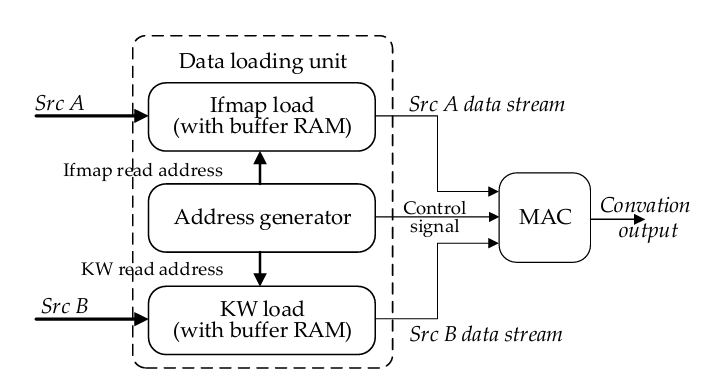
\includegraphics[width=0.5\textwidth]{Images/CNNAccelerator/CompactCNNAccelerator/conv_architecture.png}
    \vspace{10pt} % Thay đổi giá trị 10pt theo nhu cầu
    \caption{Kiến trúc của khối tích chập}
\end{figure}
Flow hoạt động của khối tích chập được thể hiện ở hình bên dưới:
\begin{figure}[!h]
    \centering
    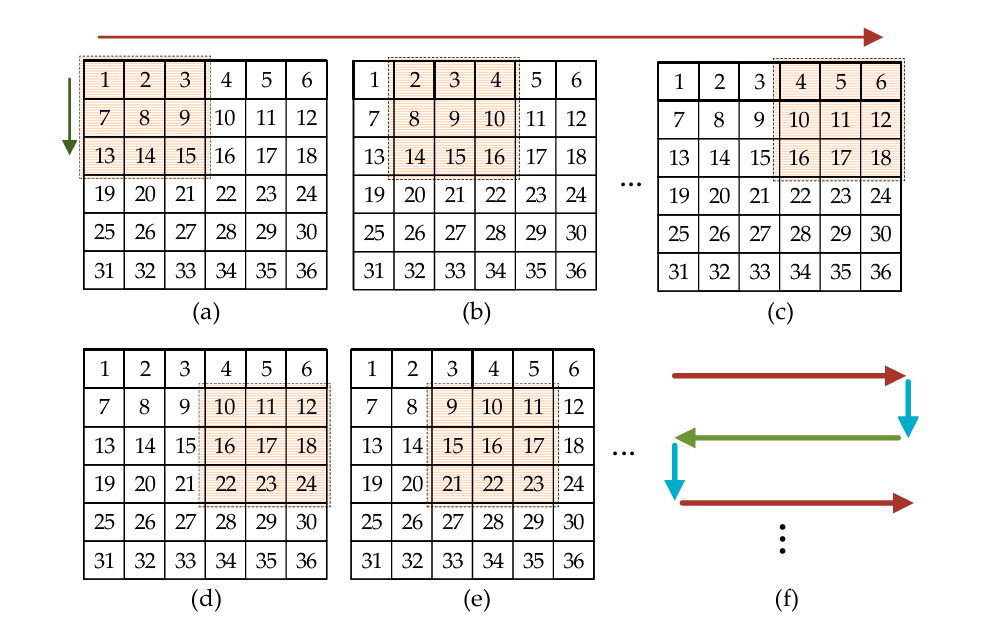
\includegraphics[width=0.7\textwidth]{Images/CNNAccelerator/CompactCNNAccelerator/conv_workflow.png}
    \vspace{10pt} % Thay đổi giá trị 10pt theo nhu cầu
    \caption{Workflow của khối tích chập}
\end{figure}

\begin{itemize}
    \item Đây là thành phần quan trọng nhất trong bộ gia tốc CNN vì CNN chủ yếu sử dụng phép toán tích chập. Thiết kế của đơn vị tích chập tập trung vào tối ưu hóa việc tải và lưu trữ dữ liệu.
    \item Sử dụng kỹ thuật giảm băng thông bộ nhớ bằng cách tận dụng sự lặp lại của dữ liệu trong phép toán tích chập, giúp giảm bớt băng thông cần thiết và tăng tốc độ tính toán.
    \item Các tín hiệu đầu vào được xử lý qua một bộ nhớ đệm (buffer RAM) để tối ưu hóa việc truy xuất dữ liệu.
\end{itemize}
\subsubsection{Khối Pooling}
Kiến trúc tổng quát của khối max-pooling được thể hiện ở sơ đồ bên dưới: 
\begin{figure}[!h]
    \centering
    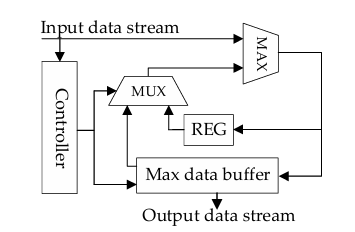
\includegraphics[width=0.5\textwidth]{Images/CNNAccelerator/CompactCNNAccelerator/pooling_architecture.png}
    \vspace{10pt} % Thay đổi giá trị 10pt theo nhu cầu
    \caption{Kiến trúc của khối pooling}
\end{figure}
\begin{itemize}
    \item Khối max-pooling thực hiện phương pháp max-pooling, giúp giảm kích thước dữ liệu đầu ra sau khi qua phép toán tích chập.
    \item Thiết kế của khối max-pooling là một mạch nối tiếp với bộ chọn và bộ so sánh (max comparator), cho phép giảm thiểu tài nguyên nhưng vẫn đảm bảo hiệu năng tính toán.
\end{itemize}
\subsubsection{Khối Multifunctional Accumulation Unit}
 Khối này được sử dụng để tích lũy kết quả của nhiều phép tích chập 2D. Nó cũng được chia sẻ với lớp bias, đơn giản hóa thiết kế và giảm tiêu thụ tài nguyên.
\subsubsection{Thiết kế chuỗi tăng tốc}
Chuỗi tăng tốc được thể hiện ở sơ đồ bên dưới:
\begin{figure}[!h]
    \centering
    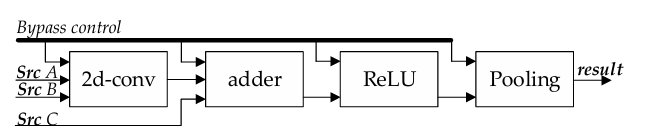
\includegraphics[width=0.5\textwidth]{Images/CNNAccelerator/CompactCNNAccelerator/chain_architecture.png}
    \vspace{10pt} % Thay đổi giá trị 10pt theo nhu cầu
    \caption{Kiến trúc của chuỗi tăng tốc}
\end{figure}
Bộ tăng tốc CNN được thiết kế theo dạng chuỗi gia tốc để tối ưu hóa hiệu suất tính toán. Mỗi chuỗi tăng tốc có thể thực hiện nhiều phép toán cùng lúc, giảm bớt sự di chuyển của dữ liệu giữa các phép toán và tăng hiệu suất tính toán. Cấu trúc của chuỗi tăng tốc bao gồm:
\begin{itemize}
    \item 4 chuỗi tăng tốc (acceleration chains): Mỗi chuỗi có thể thực hiện một phép toán tích chập độc lập, đồng thời giảm thiểu sự trùng lặp trong việc sử dụng tài nguyên.
    \item Kênh dữ liệu (Data Channels): Mỗi chuỗi gia tốc sử dụng các kênh dữ liệu như Src A, Src B, Src C, và kênh kết quả để chia sẻ thông tin giữa các thành phần khác nhau của bộ gia tốc.
\end{itemize}
Thiết kế này giúp xử lý song song nhiều lớp CNN với hiệu suất cao, đồng thời tiết kiệm tài nguyên bộ nhớ và giảm tiêu thụ năng lượng.\\
Bộ tăng tốc sử dụng một hệ thống điều khiển bypass để bỏ qua các module không cần thiết trong mỗi lớp mạng CNN, nhằm tối ưu hóa tốc độ xử lý. Các phép toán cũng được điều chỉnh độ rộng dữ liệu để phù hợp với kiến trúc 10-bit fixed-point, điều này giúp tiết kiệm tài nguyên mà không ảnh hưởng lớn đến độ chính xác. Bảng bên dưới cho thấy ảnh hưởng của độ rộng dữ liệu đối với độ chính xác của thuật toán là không đáng kể.
\subsubsection{Kiến trúc bộ tăng tốc}
Kiến trúc tổng quát của bộ tăng tốc được thể hiện ở sơ đồ bên dưới:
\begin{figure}[!h]
    \centering
    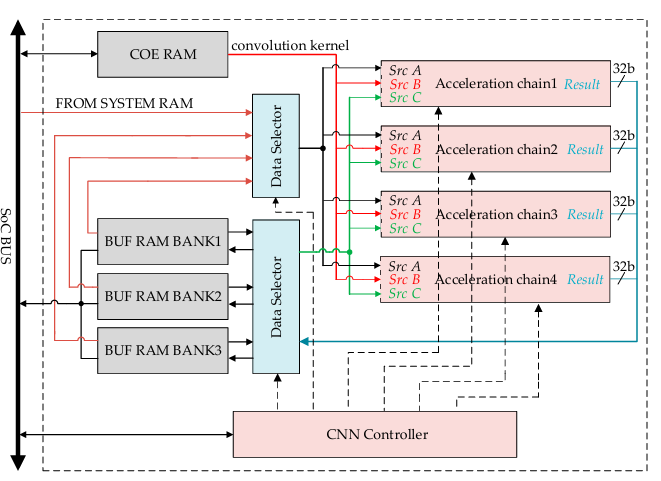
\includegraphics[width=0.7\textwidth]{Images/CNNAccelerator/CompactCNNAccelerator/accelerator_architecture.png}
    \vspace{10pt} % Thay đổi giá trị 10pt theo nhu cầu
    \caption{Kiến trúc của bộ tăng tốc}
\end{figure}
\begin{itemize}
    \item Bộ tăng tốc bao gồm bộ điều khiển CNN, ba khối đệm, bốn chuỗi tăng tốc và bộ chọn dữ liệu.
    \item Kiến trúc cho phép bộ tăng tốc thực hiện đồng thời các phép tích chập, kích hoạt và lấy mẫu con với bốn nhân tích chập dựa trên việc sử dụng ma trận nguồn, tăng hiệu suất tính toán.
    \item Bộ nhớ BUF RAM BANK được sử dụng để lưu trữ psum, ma trận nguồn và kết quả đệm, giảm thiểu việc di chuyển dữ liệu và tăng hiệu suất hệ thống. Mỗi BUF RAM BANK được ghép nối từ bốn SP-RAM độc lập để tăng băng thông truy cập.
    \item Bảng bên dưới tóm tắt các thông số cơ bản của bộ tăng tốc, cho thấy nó có thể đáp ứng các yêu cầu nhận dạng hình ảnh chung của SoC đầu cuối IoT.
\end{itemize}
\subsubsection{Thực nghiệm}
Để kiểm tra tính khả thi và hiệu quả của bộ gia tốc thiết kế, nhóm tác giả đã thực hiện một loạt thử nghiệm trên nền tảng FPGA, mô phỏng một hệ thống SoC (System-on-Chip) với bộ xử lý Cortex-M3.\\
Nền tảng thử nghiệm sử dụng vi xử lý ARM Cortex-M3 và chạy mạng Lenet-5 làm ví dụ.. Các thành phần chính của nền tảng thử nghiệm bao gồm:
\begin{itemize}
    \item Nền tảng được xây dựng dựa trên lõi Cortex-M3, một lõi MCU phổ biến của ARM cung cấp sự cân bằng tốt giữa hiệu suất và mức tiêu thụ năng lượng.
    \item SoC thử nghiệm bao gồm 128 KB RAM, 128 KB ROM và các thiết bị ngoại vi thông thường như GPIO và UART.
    \item SoC sử dụng bus AHB và APB để kết nối các thiết bị với lõi, với các thiết bị tốc độ cao như SCCB và bộ tăng tốc CNN được kết nối thông qua bus AHB, trong khi các thiết bị tốc độ thấp như GPIO được kết nối thông qua bus APB.
    \item Bảng dưới cho thấy mức tiêu thụ tài nguyên LUT của SoC khi được tổng hợp và triển khai trên FPGA. Bộ tăng tốc CNN chiếm 4901 LUT, chiếm tỷ lệ đáng kể trong tổng mức tiêu thụ tài nguyên của SoC.
\end{itemize}
Triển khai mạng kiểm thử Lenet-5
\begin{itemize}
    \item Mạng Lenet-5 được sử dụng để đánh giá bộ tăng tốc CNN. Lenet-5 là một mạng CNN cổ điển với các lớp tích chập (convolution layers), lớp gộp (subsampling), và lớp kết nối đầy đủ (fully connected). Việc triển khai mạng Lenet-5 trên nền tảng thử nghiệm giúp kiểm tra khả năng của bộ gia tốc trong việc xử lý các tác vụ nhận diện hình ảnh.
\end{itemize}
Kết quả thực nghiệm:
\begin{itemize}
    \item Hiệu suất của bộ tăng tốc được so sánh với CPU Intel i5 7500 và hai bộ xử lý ứng dụng di động Samsung S5P6818 và AllWinner H3
    \item Thời gian thực thi của Lenet-5 được đo trên các nền tảng khác nhau và được hiển thị ở bên dưới:
    \begin{figure}[!h]
    \centering
    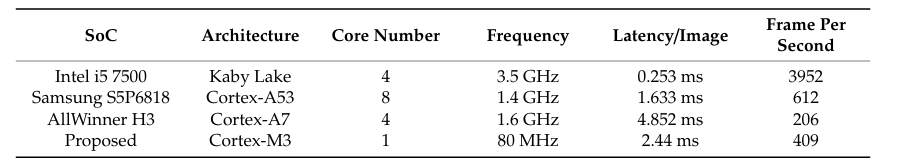
\includegraphics[width=\textwidth]{Images/CNNAccelerator/CompactCNNAccelerator/performance_table.png}
    \vspace{10pt} % Thay đổi giá trị 10pt theo nhu cầu
    \caption{Hiệu năng}
\end{figure}
\end{itemize}
Mức tiêu thụ tài nguyên:
Bài báo so sánh mức tiêu thụ tài nguyên của bộ tăng tốc được đề xuất với các bộ tăng tốc khác được báo cáo trong các tài liệu tham khảo:
\begin{itemize}
    \item Zhang, Y.; Wu, N.; Zhou, F.; Yahya, M.R. Design of Multifunctional Convolutional Neural Network Accelerator for IoT Endpoint SoC. In Proceedings of the World Congress on Engineering and Computer Science 2018, San Francisco, CA, USA, 23–25 October 2018; pp. 16–19.
    \item  Li, Z.; Wang, L.; Guo, S.; Deng, Y.; Dou, Q.; Zhou, H.; Lu, W. Laius: An 8-bit fixed-point CNN hardware inference engine. In Proceedings of the 2017 IEEE International Symposium on Parallel and Distributed Processing with Applications and 2017 IEEE International Conference on Ubiquitous Computing and Communications (ISPA/IUCC), Guangzhou, China, 12–15 December 2017; pp. 143–150.
    \item  Guo,K.; Sui, L.; Qiu, J.; Yu, J.; Wang, J.; Yao, S.; Han, S.; Wang, Y.; Yang, H. Angel-Eye: A complete design flow for mapping CNN onto embedded FPGA. IEEETrans. Comput. Des. Integr. Circuits Syst. 2018, 37, 35–47.
\end{itemize}
Kết quả được hiển thị ở bảng bên dưới:
\begin{figure}[!h]
    \centering
    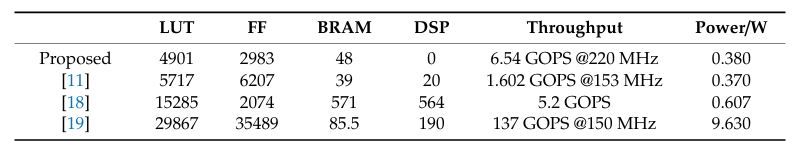
\includegraphics[width=0.7\textwidth]{Images/CNNAccelerator/CompactCNNAccelerator/resource_consumption_table.png}
    \vspace{10pt} % Thay đổi giá trị 10pt theo nhu cầu
    \caption{Mức tiêu thụ tài nguyên}
\end{figure}





\subsection{Optimization of Compiler-Generated OpenCL CNN Kernels and runtime for FPGAs}
\subsubsection{Triển khai mạng đầu cuối}
Sơ đồ luồng biên dịch được thể hiện ở hình bên dưới:
\begin{figure}[!h]
    \centering
    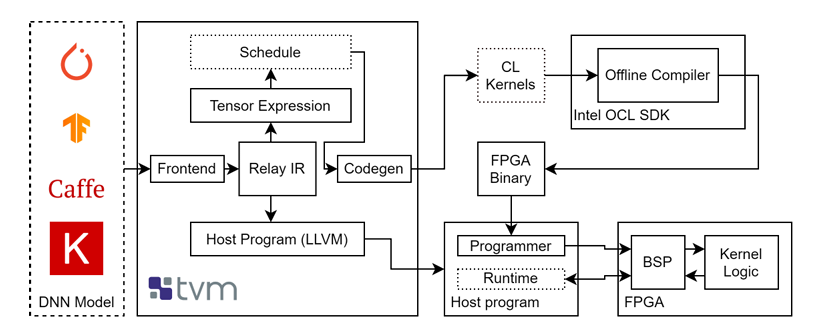
\includegraphics[width=\textwidth]{Images/CNNAccelerator/OptimizingCompiler-GeneratedOpenCLforCNNs/compilation_flow.png}
    \vspace{10pt} % Thay đổi giá trị 10pt theo nhu cầu
    \caption{Sơ đồ luồng biên dịch}
\end{figure}
\begin{itemize}
    \item Đầu vào: Mô hình CNN từ các framework ML khác nhau.
    \item TVM - một công cụ biên dịch tối ưu hóa cho học sâu, chuyển đổi mô hình thành biểu diễn trung gian (Relay IR).
    \item Biên dịch: TVM tạo mã OpenCL C từ Relay IR, sử dụng các hàm tính toán và lịch biểu được tối ưu hóa từ TVM Operator Inventory (TOPI).
    \item Tổng hợp: Intel OpenCL SDK tổng hợp mã OpenCL C thành phần cứng FPGA.
    \item Thực thi: Luồng dữ liệu được tạo trên FPGA để thực thi mô hình CNN.
\end{itemize}
Luồng biên dịch hỗ trợ hai chế độ thực thi: thực thi theo đường ống (pipelined) và thực thi gấp (folded).
\begin{itemize}
    \item Thực thi theo đường ống: Các bản đồ đặc trưng đầu ra được chuyển giữa các kernel bằng cách sử dụng các kênh OpenCL.
    \item Thực thi gấp: Các kernel được tham số hóa (hình dạng tensor đầu vào/đầu ra động) được sử dụng lại cho nhiều lớp trong mạng, tiêu thụ ít tài nguyên FPGA hơn so với thiết kế đường ống đầy đủ.
\end{itemize}
\subsubsection{Tối ưu hóa kernel OpenCL}
Các vấn đề với kernel OpenCL được tạo bởi trình biên dịch TVM:
\begin{itemize}
    \item Sử dụng bộ nhớ toàn cục không hiệu quả: Dẫn đến hiệu suất thấp do băng thông bộ nhớ toàn cục hạn chế.
    \item Sử dụng logic không hiệu quả: Dẫn đến việc sử dụng tài nguyên cao, làm cho các thiết kế lớn hơn không thể tổng hợp được.
    \item Tính song song thấp: Dẫn đến hiệu suất kém.
\end{itemize}
Các biện pháp tối ưu hóa được đề xuất:
\begin{itemize}
    \item Đọc coalesced: Kết hợp nhiều lần đọc nhỏ thành các lần đọc rộng hơn, cải thiện việc sử dụng băng thông bộ nhớ toàn cục.
    \item Lặp unrolling: Nhân rộng thân vòng lặp để tăng tính song song.
    \item Lặp fusion: Kết hợp nhiều vòng lặp thành một vòng lặp để giảm chi phí điều khiển vòng lặp và cải thiện cục bộ bộ nhớ cache.
    \item Di chuyển mã bất biến: Di chuyển các tính toán bất biến ra khỏi vòng lặp để giảm chi phí tính toán.
    \item Ghi bộ nhớ cache: Ghi kết quả trung gian vào bộ nhớ cục bộ để giảm truy cập bộ nhớ toàn cục.
    \item Kênh: Sử dụng kênh OpenCL để truyền dữ liệu giữa các kernel, giảm chi phí truyền dữ liệu bộ nhớ toàn cục và tăng tính song song.
    \item Kernel Autorun: Cho phép các kernel không có trọng số hoặc độ lệch thực thi ngay khi bộ đệm đầy, tăng tính song song.
    \item Thực thi đồng thời: Sử dụng nhiều hàng đợi lệnh để cho phép các kernel chạy song song, tăng hiệu suất.
    \item Kernel được tham số hóa: Nhóm và tham số hóa các kernel tương tự để chúng có thể được sử dụng lại trên toàn mạng, giảm mức sử dụng tài nguyên.
    \item Tối ưu hóa hoạt động dấu phẩy động: Sử dụng các tối ưu hóa do Intel OpenCL SDK cung cấp để cải thiện hiệu suất của các hoạt động dấu phẩy động.
\end{itemize}
Các phương pháp tối ưu hóa và khả năng áp dụng của chúng được thể hiện ở hình bên dưới.
\begin{figure}[!h]
    \centering
    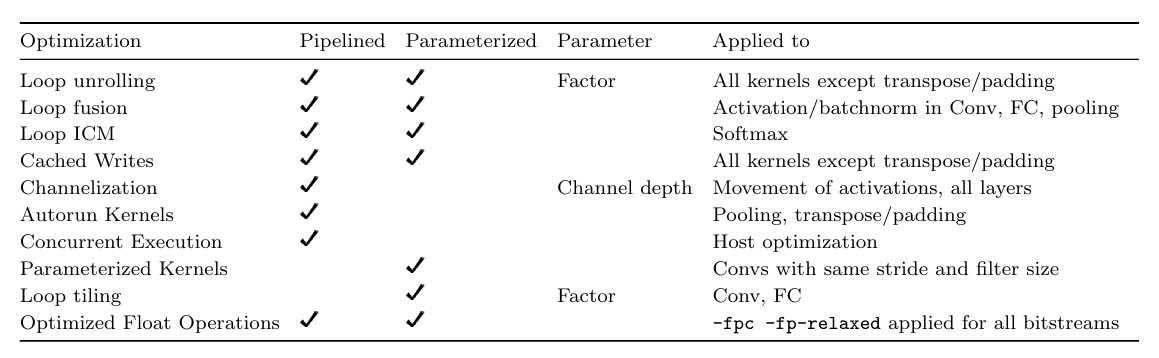
\includegraphics[width=\textwidth]{Images/CNNAccelerator/OptimizingCompiler-GeneratedOpenCLforCNNs/optimization_summary.png}
    \vspace{10pt} % Thay đổi giá trị 10pt theo nhu cầu
    \caption{Các phương pháp tối ưu hóa và khả năng áp dụng của chúng}
\end{figure}
\subsubsection{Triển khai}
\paragraph{Schedule Optimization}
\begin{itemize}
    \item Lớp Convolution: Schedule được tối ưu hóa bao gồm unrolling vòng lặp giảm, tiling dọc theo kênh FM đầu vào và cột FM đầu ra và unrolling các vòng lặp bên trong.
    \item Lớp fully-connected (FC): Lịch biểu được tối ưu hóa liên quan đến việc khai thác vòng lặp bên trong để tối đa hóa việc sử dụng bộ nhớ toàn cục và unrolling vòng lặp bên trong.
    \item Lớp Softmax: Lịch biểu được tối ưu hóa bao gồm việc kết hợp các vòng lặp để tính toán giá trị tối đa và tổng hàm mũ.
\end{itemize}
\paragraph{Custom Host Code}
Một chương trình máy chủ OpenCL C/C++ được triển khai bên ngoài TVM để hỗ trợ các tối ưu hóa không được hỗ trợ trong mã tạo máy chủ TVM.
\paragraph{Symbolic Shape Execution}
Tính năng này được sử dụng để nhóm việc thực thi các phép chập có cùng bước và kích thước bộ lọc vào cùng một kernel, cho phép sử dụng lại kernel và giảm mức sử dụng tài nguyên.
\subsubsection{Đánh giá}
\paragraph{Phương pháp}
\begin{itemize}
    \item Ba mạng CNN (LeNet-5, MobileNetV1 và ResNet-18/34) được triển khai trên ba nền tảng FPGA (Intel Arria 10, Stratix 10 MX và Stratix 10 SX).
    \item Hiệu suất được so sánh với các triển khai được tối ưu hóa cao trên CPU và GPU.
    \item Các chỉ số hiệu suất bao gồm FPS (Frames per second), GFLOPS (Floating-point operations per second) và mức sử dụng tài nguyên.
\end{itemize}
\paragraph{Nền tảng}
Thực hiện thí nghiệm với 3 nền tảng sau:
\begin{itemize}
    \item FPGA: Intel Arria 10 GX, Stratix 10 SX và Stratix 10 MX.
    \item CPU: Intel Xeon Platinum 8280.
    \item GPU: NVIDIA GTX 1060.
\end{itemize}
\paragraph{Hiệu suất suy luận}
\textbf{LeNet-5}:
Kết quả được hiển thị ở bên dưới:
\begin{figure}[!h]
    \centering
    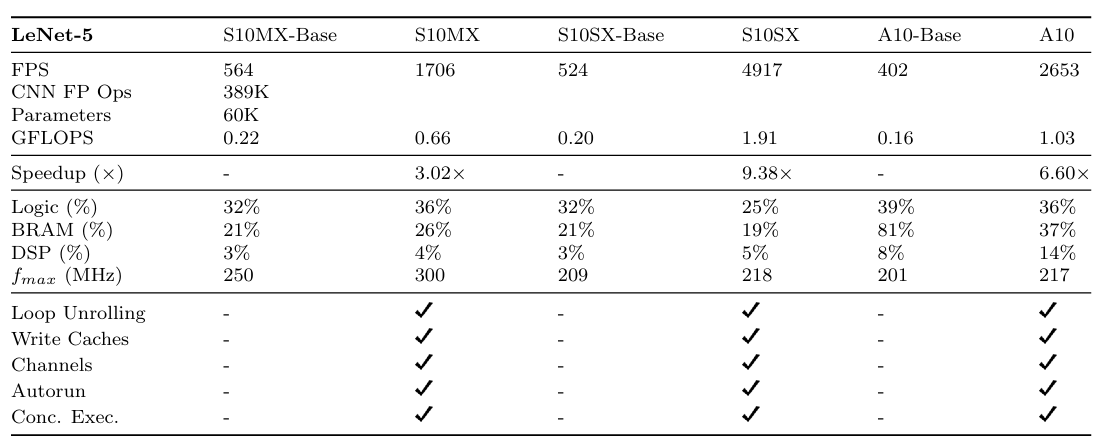
\includegraphics[width=\textwidth]{Images/CNNAccelerator/OptimizingCompiler-GeneratedOpenCLforCNNs/lenet5_inference.png}
    \vspace{10pt} % Thay đổi giá trị 10pt theo nhu cầu
    \caption{Kết quả khi hiện thực LeNet-5}
\end{figure}
\begin{itemize}
    \item FPGA đạt hiệu suất từ 1.59$\times$ đến 4.57$\times$ so với TF-CPU, 0.73$\times$ đến 2.10$\times$ so với TVM-1T và 1.06$\times$ đến 3.07$\times$ so với TF-cuDNN.
    \item Kết luận: Các bitstream FPGA được tối ưu hóa mang lại hiệu năng vượt trội so với CPU và cạnh tranh với GPU.
\end{itemize}
\textbf{MobileNetV1}
Kết quả được hiển thị ở bên dưới:
\begin{figure}[!h]
    \centering
    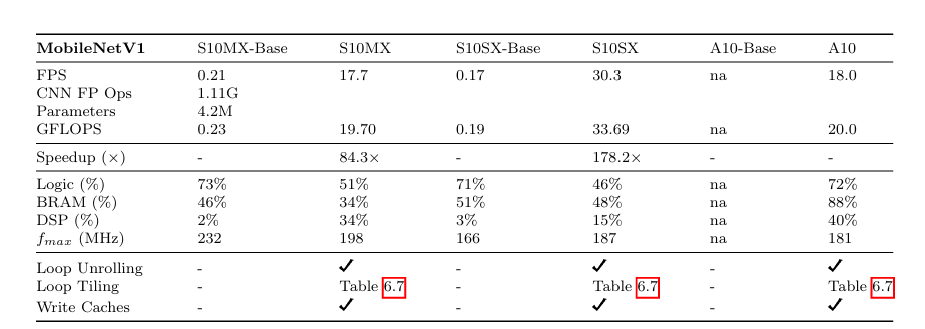
\includegraphics[width=\textwidth]{Images/CNNAccelerator/OptimizingCompiler-GeneratedOpenCLforCNNs/mobilenet.png}
    \vspace{10pt} % Thay đổi giá trị 10pt theo nhu cầu
    \caption{Kết quả khi hiện thực MobileNetV1}
\end{figure}
\begin{itemize}
    \item FPGA đạt hiệu suất từ 0.82$\times$ đến 1.40$\times$ so với TF-CPU, 1.13$\times$ đến 1.94$\times$ so với TVM-1T và chậm hơn từ 0.41$\times$ đến 0.69$\times$ so với TF-cuDNN.
    \item Kết luận: FPGA mang lại hiệu năng cạnh tranh với CPU và chậm hơn GPU, hiệu suất bị giới hạn bởi việc sử dụng DSP thấp và hiệu suất của các lớp khác.
\end{itemize}
\textbf{ResNet}
Kết quả được hiển thị ở bên dưới:
\begin{figure}[!h]
    \centering
    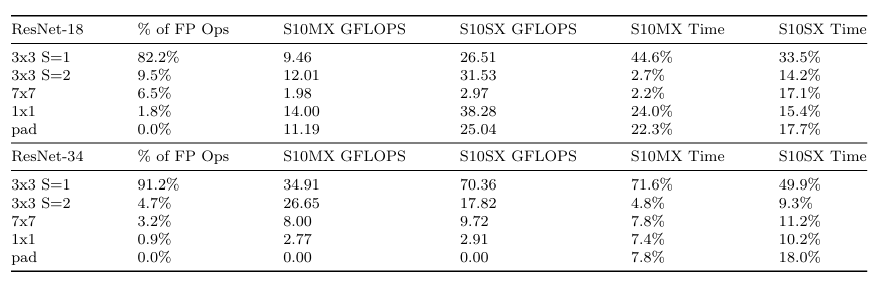
\includegraphics[width=\textwidth]{Images/CNNAccelerator/OptimizingCompiler-GeneratedOpenCLforCNNs/resnet.png}
    \vspace{10pt} % Thay đổi giá trị 10pt theo nhu cầu
    \caption{Kết quả khi hiện thực ResNet}
\end{figure}
\begin{itemize}
    \item FPGA chậm hơn CPU và GPU.
    \item Kết luận: Hiệu suất bị giới hạn bởi việc sử dụng DSP thấp và hiệu suất của các lớp khác.
\end{itemize}
\subsubsection{Hạn chế}
\begin{itemize}
    \item Sử dụng khối DSP thấp: Việc triển khai bị giới hạn bởi khả năng sử dụng DSP tối đa đạt được, đặc biệt là đối với các mạng lớn hơn.
    \item Suy giảm Fmax: Việc lát gạch và trải cuộn vòng lặp có thể dẫn đến suy giảm fmax do tăng độ phức tạp của việc định tuyến.
    \item Hiệu suất của các lớp khác: Hiệu suất của các phép cuộn 3x3 chiều sâu, đệm, softmax, và các lớp dày đặc hiện đang giới hạn hiệu suất tổng thể.
\end{itemize}
\section{Kiến trúc tăng tốc CNN gắn với RISC-V}
\subsection{RoCC, DMA và tổ chức GEMM}
Nghiên cứu của He là đối chiếu chính về đường tích hợp CPU--accelerator. Phần kiến trúc mô tả Rocket Core kết nối bộ tăng tốc qua RoCC; bộ tăng tốc dùng DMA để đọc/ghi feature map qua L2 cache và DRAM. Khối điều khiển, khối tính toán và khối lưu trữ cục bộ cho phép phân biệt việc phát lệnh của CPU với di chuyển dữ liệu của phần cứng~\cite[Section~3, Figure~4]{he2021design}. Khác với cơ chế này, trong MyTinyMobileNetSoC, CPU phải đọc tensor rồi ghi toán hạng qua MMIO; ngoại vi không có đường DMA tới RAM.

Khối tính toán của He kết hợp GEMM với mảng systolic giữ trọng số tại các phần tử xử lý (weight-stationary). Các PE hợp thành tile; thanh ghi giữa các tile tổ chức đường ống. Trọng số được nạp trước rồi dùng với luồng đầu vào, trong khi chia khối phép nhân ma trận nhằm giảm truy cập lặp~\cite[Sections~2.2--3, Figure~5]{he2021design}. Phạm vi mô tả tập trung vào tăng tốc tích chập bằng tính toán ma trận; sơ đồ có khối activation/pooling, nhưng bài không mô tả đủ để xác nhận một đường depthwise chuyên biệt hoặc toàn bộ hậu xử lý giống firmware của luận văn.

Đặt cạnh thiết kế này, Conv/Depthwise/Pointwise của MyTinyMobileNetSoC biểu diễn các phép tính theo cấu trúc toán tử thay vì một mảng GEMM chung. Firmware quyết định khi nào giữ patch, nạp trọng số và sử dụng kết quả cho từng shape. Phương án ma trận có thể dùng chung lõi tính toán cho nhiều lớp, đổi lại yêu cầu ánh xạ tensor và cấp dữ liệu đủ đều. Phương án chuyên biệt giảm nhu cầu ánh xạ qua ma trận trong đường chạy hiện tại, nhưng có phạm vi shape và các nhánh fallback phải kiểm chứng. Hai cách tổ chức đặt sự phức tạp ở những vị trí khác nhau.

\subsection{Giới hạn bằng chứng và ý nghĩa đối chiếu}
Phần thực nghiệm của He sử dụng YOLOv3-tiny và báo cáo thời gian xử lý trên nền tảng FPGA~\cite[Section~4]{he2021design}. Tuy nhiên, sơ đồ kiến trúc ghi Rocket Core còn phần kết luận nêu BOOM hai lõi. Vì thế, chương chỉ dùng Rocket/RoCC để chỉ phương án kết nối được mô tả, không coi đây là cấu hình host đã được xác nhận nhất quán cho toàn bộ số đo. Bài cũng không công bố rõ độ rộng toán hạng và tích lũy của cấu hình đánh giá, nên không gán INT8/INT32 cho thiết kế này.

Sự khác nhau về workload, host và hệ thống nhớ không cho phép xếp hạng từ FPS được báo cáo. Giá trị đối chiếu nằm ở mức tự chủ: với DMA, CPU có thể giao tác vụ có kích thước lớn hơn cho accelerator; với MMIO do CPU cấp dữ liệu, chi phí mỗi lần gọi và lượng dữ liệu hữu ích mỗi giao dịch trở thành mục tiêu tối ưu trực tiếp. Đây là cơ sở để Chương~\ref{chap:kientruc} làm rõ ranh giới giao diện và Chương~\ref{chap:toiuu} đánh giá cả phần truyền dữ liệu của MyTinyMobileNetSoC.

\section{Hướng tăng tốc tổng quát bằng mảng systolic/GEMM}
ConvAU của Kiningham, Graczyk và Ramkumar đại diện cho hướng lấy nhân ma trận đặc làm trung tâm. Thiết kế dùng phép nhân 8 bit và tích lũy 32 bit, giữ trọng số tại PE, cấp đầu vào qua FIFO SRAM và lưu kết quả trung gian trong hệ thống đệm. Host nạp trọng số cùng metadata lượng tử hóa; phần cứng đảm nhiệm tính toán ma trận, lượng tử hóa và ReLU. Báo cáo không xác định một lõi RISC-V hoặc giao thức MMIO/RoCC tương ứng, nên không thể xem ConvAU là một SoC cùng cấu hình với luận văn~\cite[Sections~3--4]{kiningham2016design}.

\subsection{Thông lượng, chuẩn bị dữ liệu và mức sử dụng mảng}
Dòng MAC đều đặn cho phép tái sử dụng toán hạng qua các PE và khai thác song song khi kích thước ma trận phù hợp. Tuy nhiên, tích chập cần được ánh xạ sang phép nhân ma trận. ConvAU trình bày phép biến đổi im2col để sắp cửa sổ đầu vào thành cột~\cite[Section~4.2]{kiningham2016design}. Nếu vật chất hóa ma trận đó, các phần tử cửa sổ chồng lấn bị lặp, làm tăng lưu trữ và lưu lượng; nếu sinh dữ liệu theo luồng, chi phí chuyển sang bộ tạo địa chỉ và bộ đệm. Vì vậy, so sánh phải tính cả chuẩn bị dữ liệu, nạp trọng số, làm đầy và tháo cạn đường ống.

Đối với workload của luận văn, pointwise có cấu trúc trộn kênh phù hợp phép nhân ma trận, còn depthwise tính độc lập từng kênh~\cite[Section~3.1]{howard2017mobilenets}. Từ cấu trúc đó có thể suy ra rằng ánh xạ depthwise hoặc ma trận nhỏ lên mảng đặc lớn cần lịch ghép tác vụ hay chia khối phù hợp để tránh nhiều PE không có việc hữu ích. Đây là nhận xét về điều kiện sử dụng mảng, không phải số đo mức sử dụng của ConvAU trên TinyMobileNet và cũng không có nghĩa mọi mảng systolic đều xử lý depthwise kém.

\subsection{Phạm vi đánh giá và bài học cho hệ thống hiện tại}
ConvAU được đánh giá bằng RTL, tổng hợp và luồng ASIC, với SqueezeNet lượng tử hóa làm workload~\cite[Section~5]{kiningham2016design}. Thông lượng và công suất trong báo cáo thuộc điều kiện đó; không dùng chúng để suy ra ưu thế năng lượng hoặc độ trễ của FPGA trong luận văn. So sánh số bit cũng chỉ là một tiêu chí: cùng độ rộng tensor và tích lũy chưa bảo đảm quy tắc làm tròn hay saturation giống nhau.

Khác với ConvAU, MyTinyMobileNetSoC không thực hiện mạng bằng một mảng ma trận đặc chung và không dựng ma trận im2col đầy đủ trong đường chạy hiện tại. Dữ liệu được chuẩn bị theo patch hoặc vector kênh cho ngoại vi chuyên biệt. Lựa chọn này phù hợp phạm vi hiện thực TinyMobileNet đã xác định, nhưng đánh đổi bằng lịch firmware phụ thuộc shape và phần tính toán còn ở CPU. Bài học từ hướng systolic là phải cân đối số MAC với khả năng nuôi dữ liệu và miền tái sử dụng, thay vì xem kích thước mảng là thước đo đủ cho hiệu năng hệ thống.

\section{Tổng hợp so sánh và vị trí của MyTinyMobileNetSoC}
\label{sec:related-position}
Bảng~\ref{tab:related-integration} và Bảng~\ref{tab:related-scope} dùng cùng tập công trình để đối chiếu hai nhóm tiêu chí: tích hợp/luồng dữ liệu và phạm vi/số học. Các nhận xét ở cột cuối là tổng hợp kiến trúc của chương; chúng không biểu thị thứ hạng. Khi nguồn không xác định rõ một thuộc tính, bảng ghi giới hạn đó thay vì suy đoán từ tên nền tảng.

\begingroup
\small
\setlength{\tabcolsep}{4pt}
\renewcommand{\arraystretch}{1.12}
\begin{longtable}{@{}>{\raggedright\arraybackslash}p{0.17\textwidth}>{\raggedright\arraybackslash}p{0.23\textwidth}>{\raggedright\arraybackslash}p{0.28\textwidth}>{\raggedright\arraybackslash}p{0.26\textwidth}@{}}
\caption{So sánh host, kiểu tăng tốc và truyền dữ liệu}\label{tab:related-integration}\\
\toprule
Công trình & CPU/host và kiểu tăng tốc & Điều khiển, truyền dữ liệu & Miền tái sử dụng chính \\
\midrule
\endfirsthead
\toprule
Công trình & CPU/host và kiểu tăng tốc & Điều khiển, truyền dữ liệu & Miền tái sử dụng chính \\
\midrule
\endhead
\bottomrule
\endfoot
Ge và cộng sự~\cite{ge2019compact} & Cortex-M3; chuỗi tích chập, kích hoạt, pooling & AHB tới accelerator; điều khiển và bank nhớ nội bộ & Buffer cửa sổ; chia sẻ nguồn giữa chuỗi; bank luân phiên giữ tổng riêng/kết quả \\
\midrule
He~\cite{he2021design} & Sơ đồ Rocket; GEMM/systolic giữ trọng số & RoCC điều khiển; DMA tới L2/DRAM & Trọng số tại PE; tile ma trận và lưu trữ cục bộ \\
\midrule
ConvAU~\cite{kiningham2016design} & Host không xác định lõi; mảng nhân ma trận đặc & Host nạp trọng số/metadata; không xác định giao thức bus SoC & Trọng số tại PE; FIFO đầu vào và đệm trung gian \\
\midrule
Chung~\cite{chung2021optimization} & Host OpenCL; kernel FPGA sinh từ TVM & Runtime, buffer toàn cục, hàng đợi; kênh giữa kernel khi pipeline & Tiling, lưu cục bộ, fusion và tái dùng kernel khi folded \\
\midrule
MyTiny\-Mobile\-NetSoC (Chương~\ref{chap:kientruc}) & PicoRV32; ngoại vi Conv, Depthwise, Pointwise, Quant & MMIO qua bus gốc; CPU chuyển toán hạng; không DMA; RAM mã/dữ liệu 256~KiB & Patch/tile và cache trọng số chuyên biệt, do firmware lập lịch theo shape \\
\end{longtable}
\endgroup

\begingroup
\small
\setlength{\tabcolsep}{4pt}
\renewcommand{\arraystretch}{1.12}
\begin{longtable}{@{}>{\raggedright\arraybackslash}p{0.17\textwidth}>{\raggedright\arraybackslash}p{0.18\textwidth}>{\raggedright\arraybackslash}p{0.26\textwidth}>{\raggedright\arraybackslash}p{0.33\textwidth}@{}}
\caption{So sánh số học, phạm vi đánh giá và khác biệt với luận văn}\label{tab:related-scope}\\
\toprule
Công trình & Số học & Phạm vi và bằng chứng & Khác biệt chính so với luận văn \\
\midrule
\endfirsthead
\toprule
Công trình & Số học & Phạm vi và bằng chứng & Khác biệt chính so với luận văn \\
\midrule
\endhead
\bottomrule
\endfoot
Ge và cộng sự~\cite{ge2019compact} & Fixed-point 10 bit; tổng riêng 32 bit & SoC FPGA; đánh giá LeNet-5 & Nhiều bước xử lý và buffering nằm trong accelerator; không xác nhận đường depthwise riêng \\
\midrule
He~\cite{he2021design} & Không nêu rõ độ rộng cấu hình đánh giá & FPGA; YOLOv3-tiny; phần kết luận nêu BOOM khác host trong sơ đồ & Tập trung nhân ma trận và DMA; không đủ chi tiết để đồng nhất cấu hình số học/host của số đo \\
\midrule
ConvAU~\cite{kiningham2016design} & Nhân 8 bit; tích lũy 32 bit & RTL và luồng ASIC; SqueezeNet lượng tử hóa & Ánh xạ CNN sang ma trận; phần cứng có ReLU/lượng tử hóa; không phải đánh giá SoC FPGA cùng điều kiện \\
\midrule
Chung~\cite{chung2021optimization} & Dấu phẩy động & OpenCL FPGA; LeNet-5, MobileNetV1, ResNet & Tối ưu trình biên dịch và runtime; không cấp toán hạng từng phép qua MMIO \\
\midrule
MyTiny\-Mobile\-NetSoC (Chương~\ref{chap:kientruc}, \ref{chap:toiuu}) & Tensor INT8; tích lũy INT32 & TinyMobileNet/MNIST; mô phỏng và đánh giá FPGA post-route cho ZCU106 & Tích hợp và lịch firmware theo workload; còn fallback CPU; chưa xác nhận suy luận trên bo mạch \\
\end{longtable}
\endgroup

\subsection{Ranh giới tích hợp và phạm vi tối ưu được chọn}
Từ các đối chiếu trên, lựa chọn của luận văn là một hệ thống mà trách nhiệm truyền dữ liệu còn tường minh ở CPU. PicoRV32 đọc tensor từ RAM dùng chung, nạp các thanh ghi ngoại vi và thu kết quả. RAM 256~KiB là bộ nhớ chung cho mã và dữ liệu của CPU; các bộ tăng tốc không có cổng tự truy cập RAM. Conv, Depthwise, Pointwise và Quant là các đường được firmware sử dụng; SoC còn có bộ nhân độc lập nhưng đường suy luận hiện tại không sử dụng nó (Chương~\ref{chap:kientruc}).

Phạm vi tăng tốc không bao phủ mọi phép toán của mạng. Trong thiết kế cuối, Conv0, DW1, DW2 và các lớp Pointwise có đường tích lũy phần cứng; DW3, GAP và FC vẫn dùng số học CPU. Requantization dùng ngoại vi Quant, còn CPU chịu trách nhiệm bias, offset đầu ra, clamp và điều phối lớp. Trọng số và feature map là INT8, bias và tích lũy là INT32; điều đó không tự xác nhận tương đương từng bit với các hệ lượng tử hóa khác. Phân công cụ thể được làm rõ trong Chương~\ref{chap:kientruc}, tránh đồng nhất tên ngoại vi với mức bao phủ toàn bộ toán tử.

So với bộ đồng xử lý DMA hoặc mảng GEMM chung, phạm vi tối ưu ở đây tập trung vào giao dịch MMIO, lịch vòng lặp và lưu giữ dữ liệu theo shape của TinyMobileNet. Đổi lại, việc chuyên biệt hóa cần điều kiện chọn nhánh, fallback và kiểm tra giao dịch tương ứng. Kết quả được đánh giá bằng điểm số/dự đoán, số chu kỳ và tài nguyên/timing post-route trên mục tiêu ZCU106 ở Chương~\ref{chap:toiuu}. Flow hiện có chưa xác nhận suy luận TinyMobileNet trên bo mạch và chưa có số đo năng lượng để đối chiếu các công trình trước.

Các nghiên cứu được giữ lại làm rõ những lựa chọn đã có về phân công, lưu trữ và lập lịch; chúng không đủ cơ sở để khẳng định tính mới hoặc ưu thế phổ quát của MyTinyMobileNetSoC. Vị trí của đề tài là hiện thực và đánh giá một phương án tích hợp cụ thể, trong đó hiệu năng phụ thuộc đồng thời vào datapath chuyên biệt và cách CPU phục vụ dữ liệu. Từ những lựa chọn này, Chương~\ref{chap:kientruc} trình bày kiến trúc được chọn, giao diện MMIO và đường suy luận thực tế của hệ thống.


\newpage
\chapter{KIẾN TRÚC VÀ THIẾT KẾ HỆ THỐNG}
\label{chap:kientruc}
\section{Tổng quan phương pháp}
Đề tài hướng tới thực thi suy luận mạng nơ-ron tại thiết bị biên bằng một hệ thống kết hợp bộ xử lý RISC-V và các bộ tăng tốc chuyên dụng. Đối tượng hiện thực là MyTinyMobileNetSoC: lõi PicoRV32 điều khiển mạng TinyMobileNet sử dụng kích hoạt và trọng số INT8. Thay vì chuyển toàn bộ đồ thị suy luận thành một khối phần cứng cố định, hệ thống phân chia nhiệm vụ theo nguyên tắc đồng thiết kế phần cứng--phần mềm (HW/SW co-design). Phần cứng thực hiện các phép nhân--cộng và tái lượng tử hóa; firmware chịu trách nhiệm thứ tự lớp, địa chỉ tensor, xử lý biên và hoàn thiện đầu ra.

Cách phân chia này cho phép giữ giao diện lập trình đơn giản qua các thanh ghi ánh xạ bộ nhớ (memory-mapped I/O, MMIO). Tuy nhiên, CPU phải chuyển toán hạng từ RAM vào từng bộ tăng tốc và đọc kết quả về. Vì vậy, thời gian suy luận phụ thuộc cả chi phí tính toán lẫn chi phí truyền dữ liệu, điều khiển vòng lặp và hậu xử lý. Đây là cơ sở để đánh giá tối ưu hóa ở cấp hệ thống trong Chương~\ref{chap:toiuu}.

Phạm vi mô tả trong chương là mã nguồn hiện tại tại \texttt{RISCVAIoT/MyTinyMobileNetSoC/}, với đường suy luận sau Level~6. Kết quả mô phỏng, kết quả hiện thực vật lý và hoạt động trên bo mạch được xem là ba loại bằng chứng riêng. Thiết kế không có DMA cho các bộ tăng tốc, không có bộ tăng tốc Softmax hoặc MaxPool, và không sử dụng kiến trúc mảng systolic làm mô hình mô tả phần cứng hiện tại. Các sơ đồ được để ở dạng vị trí chờ, nhằm tránh dùng lại hình kiến trúc không còn phù hợp.

\section{Kiến trúc TinyMobileNet hiện thực}
\subsection{Cấu trúc mạng và kích thước tensor}
Mạng gồm Conv0, ba cặp depthwise--pointwise, GAP và FC. Bảng~\ref{tab:network-current} trình bày kích thước theo thứ tự cao $\times$ rộng $\times$ kênh; dữ liệu vẫn lưu theo CHW. Đây là mạng thu gọn được firmware thực thi, không phải toàn bộ MobileNetV2.

\begin{table}[!ht]
\renewcommand{\arraystretch}{1.12}
\centering
\caption{Các lớp của TinyMobileNet và phân công tính toán ở Level 6}
\label{tab:network-current}
\small
\begin{tabular}{llll}
\hline
Lớp & Đầu vào & Đầu ra & Tích lũy \\
\hline
Conv0 & $28\times28\times1$ & $28\times28\times16$ & Conv \\
DW1 & $28\times28\times16$ & $28\times28\times16$ & Depthwise \\
PW1 & $28\times28\times16$ & $28\times28\times32$ & Pointwise có cache \\
DW2 & $28\times28\times32$ & $14\times14\times32$ & Depthwise tái sử dụng \\
PW2 & $14\times14\times32$ & $14\times14\times48$ & Pointwise batch \\
DW3 & $14\times14\times48$ & $7\times7\times48$ & CPU \\
PW3 & $7\times7\times48$ & $7\times7\times64$ & Pointwise batch \\
GAP & $7\times7\times64$ & 64 phần tử & CPU \\
FC & 64 phần tử & 10 điểm số & CPU \\
\hline
\end{tabular}
\end{table}
Tái lượng tử hóa ở tất cả các lớp trong đường chạy SoC dùng bộ tăng tốc lượng tử, kể cả các lớp tích lũy trên CPU. Conv0 và DW1 dùng stride~1; DW2 và DW3 dùng stride~2 để giảm kích thước không gian. Pointwise dùng kernel $1\times1$ và stride~1. Conv0 và DW1 truyền padding trái/trên bằng một. DW2 và DW3 truyền padding trái/trên bằng không; các cửa sổ vượt biên phải/dưới được xử lý như padding bằng không. Các giá trị này được xác định từ lời gọi hàm, thay vì chú thích mô tả padding trong mã.

\subsection{Các phép toán của mạng}
Gọi $\widetilde{x}$ là kích hoạt sau khi cộng offset đầu vào và $w$ là trọng số số nguyên có dấu. Tích lũy của tích chập chuẩn cho kênh đầu ra $o$ được biểu diễn bởi
\begin{equation}
 a_{o,y,x}=b_o+\sum_c\sum_{u,v}w_{o,c,u,v}\,
 \widetilde{x}_{c,sy+u-p_y,sx+v-p_x},
\end{equation}
trong đó $s$ là stride, $p_y,p_x$ là padding. Công thức mô tả quan hệ tensor; trong firmware, vị trí ngoài biên được xử lý bằng nhánh kiểm tra chỉ số. Các đường phần cứng dùng padding bằng số nguyên không, không cộng offset vào phần tử padding.

Depthwise convolution với depth multiplier bằng một áp dụng một kernel riêng trên từng kênh:
\begin{equation}
 a_{c,y,x}=b_c+\sum_{u,v}w_{c,u,v}\,
 \widetilde{x}_{c,sy+u-p_y,sx+v-p_x}.
\end{equation}
Các kênh không phụ thuộc nhau trong bước này. Pointwise convolution kết hợp thông tin giữa các kênh tại cùng vị trí:
\begin{equation}
 a_{o,y,x}=b_o+\sum_c w_{o,c}\widetilde{x}_{c,y,x}.
\end{equation}
Cặp depthwise--pointwise tạo thành tích chập tách theo chiều sâu (depthwise-separable convolution): bước đầu xử lý không gian, bước sau trộn kênh~\cite[Section~3.1]{howard2017mobilenets}. Với kernel $K\times K$, số hạng nhân--cộng trên một vị trí lần lượt là $K^2C_{\rm in}C_{\rm out}$ đối với tích chập chuẩn và $K^2C_{\rm in}+C_{\rm in}C_{\rm out}$ đối với cặp tách. Đây là đếm toán học, không phải số chu kỳ thực thi; truyền MMIO có thể làm thay đổi thứ tự các nút thắt hiệu năng.

GAP thu gọn mỗi kênh bằng trung bình trên toàn bộ miền không gian,
\begin{equation}
 \bar{g}_c=\frac{1}{HW}\sum_{y,x}\widetilde{x}_{c,y,x},\qquad
 a_j=b_j+\sum_c w_{j,c}\widetilde{g}_c.
\end{equation}
Biểu thức thứ hai là lớp FC, ánh xạ vector đặc trưng sang điểm số phân loại. Trong GAP, CPU cộng offset đầu vào trước khi lấy trung bình, chia độ lớn tổng bằng thuật toán dịch--trừ và làm tròn độ lớn lên khi phần dư đạt ít nhất nửa số phần tử, sau đó khôi phục dấu. Giá trị trung bình này còn qua tái lượng tử hóa, offset đầu ra và clamp để tạo vector INT8 $g$ mà FC sử dụng; do đó $\bar{g}$ không phải trực tiếp là tensor đầu ra GAP. Mạng thực thi trả về điểm số trước Softmax; nhãn được chọn bằng argmax, không diễn giải điểm số INT8 là xác suất.

Hình~\ref{fig:network-placeholder} minh họa luồng tensor và phân công xử lý giữa CPU với phần cứng.

\begin{figure}[!ht]
% Local spacing: template has a negative figure caption skip.
\captionsetup{aboveskip=6pt,belowskip=0pt}
\centering
\resizebox{0.93\textwidth}{!}{\begingroup
\input{Images/tinymobilenet/styles.tex}
\begin{tikzpicture}[x=1cm,y=1cm]
\node[thesis block,text width=3.1cm,minimum height=.62cm] (n0) at (1.8,0.0) {\textbf{Input}\quad $28\times28\times1$};
\node[thesis note,anchor=west,align=left,text width=9.2cm] at (3.7,0.0) {INT8; CHW};
\node[thesis block,text width=3.1cm,minimum height=.62cm] (n1) at (1.8,-0.83) {\textbf{Conv0}\quad $28\times28\times16$};
\node[thesis note,anchor=west,align=left,text width=9.2cm] at (3.7,-0.83) {Conv HW + Quant; stride 1};
\draw[thesis arrow] (n0)--(n1);
\node[thesis block,text width=3.1cm,minimum height=.62cm] (n2) at (1.8,-1.66) {\textbf{DW1}\quad $28\times28\times16$};
\node[thesis note,anchor=west,align=left,text width=9.2cm] at (3.7,-1.66) {Depthwise HW + Quant; stride 1};
\draw[thesis arrow] (n1)--(n2);
\node[thesis block,text width=3.1cm,minimum height=.62cm] (n3) at (1.8,-2.4899999999999998) {\textbf{PW1}\quad $28\times28\times32$};
\node[thesis note,anchor=west,align=left,text width=9.2cm] at (3.7,-2.4899999999999998) {Pointwise HW + resident PW1 cache + Quant};
\draw[thesis arrow] (n2)--(n3);
\node[thesis block,text width=3.1cm,minimum height=.62cm] (n4) at (1.8,-3.32) {\textbf{DW2}\quad $14\times14\times32$};
\node[thesis note,anchor=west,align=left,text width=9.2cm] at (3.7,-3.32) {Depthwise HW reused for exact stride-2 path + Quant};
\draw[thesis arrow] (n3)--(n4);
\node[thesis block,text width=3.1cm,minimum height=.62cm] (n5) at (1.8,-4.1499999999999995) {\textbf{PW2}\quad $14\times14\times48$};
\node[thesis note,anchor=west,align=left,text width=9.2cm] at (3.7,-4.1499999999999995) {Pointwise HW batch + Quant};
\draw[thesis arrow] (n4)--(n5);
\node[thesis block,text width=3.1cm,minimum height=.62cm] (n6) at (1.8,-4.9799999999999995) {\textbf{DW3}\quad $7\times7\times48$};
\node[thesis note,anchor=west,align=left,text width=9.2cm] at (3.7,-4.9799999999999995) {CPU accumulation + Quant; stride 2};
\draw[thesis arrow] (n5)--(n6);
\node[thesis block,text width=3.1cm,minimum height=.62cm] (n7) at (1.8,-5.81) {\textbf{PW3}\quad $7\times7\times64$};
\node[thesis note,anchor=west,align=left,text width=9.2cm] at (3.7,-5.81) {Pointwise HW batch + Quant};
\draw[thesis arrow] (n6)--(n7);
\node[thesis block,text width=3.1cm,minimum height=.62cm] (n8) at (1.8,-6.64) {\textbf{GAP}\quad $64$};
\node[thesis note,anchor=west,align=left,text width=9.2cm] at (3.7,-6.64) {CPU sum / average + Quant};
\draw[thesis arrow] (n7)--(n8);
\node[thesis block,text width=3.1cm,minimum height=.62cm] (n9) at (1.8,-7.47) {\textbf{FC}\quad $10$};
\node[thesis note,anchor=west,align=left,text width=9.2cm] at (3.7,-7.47) {CPU accumulation + Quant};
\draw[thesis arrow] (n8)--(n9);

\draw[black!45] (.1,-8.2)--(13.3,-8.2);
\node[thesis title,anchor=west] at (.1,-8.65) {DW2 inset: reuse a loaded $5\times5$ patch};
\draw[step=.34,black!55] (.3,-10.7) grid (2,-9);
\node[thesis note] at (1.15,-11.05) {Input patch};
\draw[thesis arrow] (2.25,-9.85)--(3.1,-9.85);
\foreach \r in {0,1,2}{\foreach \c in {0,1,2}{
 \pgfmathtruncatemacro{\idx}{3*\r+\c}
 \ifnum\idx=0\def\shade{20}\else\ifnum\idx=2\def\shade{20}\else\ifnum\idx=6\def\shade{20}\else\ifnum\idx=8\def\shade{20}\else\def\shade{0}\fi\fi\fi\fi
 \node[thesis block,fill=black!\shade,minimum size=.48cm,inner sep=0pt] at ({3.5+.5*\c},{-9.35-.5*\r}) {\idx};
}}
\node[thesis note,text width=7.3cm,align=left,anchor=west] at (5.4,-9.9) {Nine stride-1 window results from the same patch.\\Select \textbf{0, 2, 6, 8}: window origins $(0,0)$, $(0,2)$,\\$(2,0)$, $(2,2)$ form a $2\times2$ stride-2 output tile.};

\end{tikzpicture}
\endgroup
}
\caption{Luồng tensor TinyMobileNet và phân công HW/SW; DW2 chọn bốn kết quả stride~2 từ cùng patch.}
\label{fig:network-placeholder}
\end{figure}

\section{Kiến trúc MyTinyMobileNetSoC}
SoC gồm PicoRV32, RAM dùng chung, UART, thanh ghi LED và năm ngoại vi tính toán: bộ nhân độc lập, Conv, Quant, Depthwise và Pointwise. CPU là chủ thể phát giao dịch bộ nhớ. Các bộ tăng tốc nhận toán hạng từ thanh ghi nội bộ; chúng không tự truy cập RAM. Do đó, RAM dùng chung cho mã và dữ liệu không đồng nghĩa bộ tăng tốc có cổng đọc bộ nhớ chung hay khả năng DMA.

Bus sử dụng các tín hiệu \texttt{mem\_valid}, \texttt{mem\_ready}, địa chỉ, dữ liệu đọc/ghi và byte-enable \texttt{mem\_wstrb}. Bộ giải mã trong \texttt{my\_soc.v} chọn RAM hoặc ngoại vi theo địa chỉ. Một giao dịch hoàn tất khi yêu cầu hợp lệ được đáp ứng bởi ready. Với kết quả batch của bộ tăng tốc Pointwise chưa sẵn sàng, ready bị giữ lại theo \texttt{rvalid}; CPU chờ trên bus thay vì chạy vòng polling.

Bảng~\ref{tab:mmio-current} liệt kê bản đồ địa chỉ RAM và các ngoại vi của hệ thống.

\begin{table}[!ht]
\renewcommand{\arraystretch}{1.12}
\centering
\caption{Bản đồ địa chỉ hiện tại của MyTinyMobileNetSoC}
\label{tab:mmio-current}
\begin{tabular}{ll}
\hline
Khối & Địa chỉ byte \\
\hline
RAM & \texttt{0x00000000}--\texttt{0x0003FFFF} \\
UART & \texttt{0x02000004 / 0x02000008} \\
Multiplier & \texttt{0x02000010}--\texttt{0x0200001F} \\
Conv & \texttt{0x02000100}--\texttt{0x020001FF} \\
Quant & \texttt{0x02000200}--\texttt{0x020002FF} \\
Depthwise & \texttt{0x02000300}--\texttt{0x020003FF} \\
Pointwise & \texttt{0x02000400}--\texttt{0x020007FF} \\
LED & \texttt{0x03000000} \\
\hline
\end{tabular}
\end{table}
UART có thanh ghi chia tần và dữ liệu tại hai địa chỉ tương ứng. LED cung cấp trạng thái do firmware ghi. Bộ nhân độc lập tồn tại trong SoC nhưng không được đường suy luận TinyMobileNet sử dụng; không được nhầm ngoại vi này với khả năng nhân của CPU hoặc các bộ nhân nằm trong accelerator.

Hình~\ref{fig:soc-placeholder} minh họa kiến trúc SoC và đường giao tiếp MMIO do CPU điều phối.

\begin{figure}[!ht]
% Local spacing: template has a negative figure caption skip.
\captionsetup{aboveskip=6pt,belowskip=0pt}
\centering
\resizebox{0.93\textwidth}{!}{\begingroup
\input{Images/tinymobilenet/styles.tex}
\begin{tikzpicture}[x=1cm,y=1cm]

\node[thesis sw,minimum width=5.2cm,minimum height=1.35cm] (cpu) at (3,0) {\textbf{CPU: PicoRV32}\\RV32IM build; MUL enabled, DIV disabled\\CPU mediates all operand/result transfers};
\node[thesis memory,text width=5.3cm,minimum height=1.35cm] (ram) at (10.6,0) {\textbf{Shared RAM: 256 KiB}\\Code, weights, activations, stack};
\draw[thesis transfer] (cpu)--node[thesis note,above=4pt]{R / W}(ram);
\node[thesis hw,text width=12.8cm,minimum height=.9cm] (bus) at (6.8,-2.2) {\textbf{MMIO interconnect / address decode}\\32-bit register transfers; valid / ready handshake};
\draw[thesis transfer] (cpu.south)--node[thesis note,left,align=right]{operands, control\\results}(3,-2.2+.59);
\foreach \x/\name/\id in {1.5/Conv/c,5/Quant/q,8.5/Depthwise/d,12/Pointwise/p}{
 \node[thesis hw,minimum width=2.8cm,minimum height=.9cm] (\id) at (\x,-4) {\name};
 \draw[thesis transfer] (\x,-2.79)--(\id.north);
}
\foreach \x/\name/\id in {1.5/UART/u,5/LED/l,10.25/Standalone multiplier/m}{
 \node[thesis hw,minimum width=2.8cm,minimum height=.8cm] (\id) at (\x,-5.8) {\name};
}
\draw[thesis transfer] (.45,-2.79)--(.45,-3.05)--(-.25,-3.05)--(-.25,-5.8)--(u.west);
\draw[thesis transfer] (6.6,-2.79)--(6.6,-5.8)--(l.east);
\draw[thesis transfer] (13.5,-2.79)--(13.5,-5.8)--(m.east);
\node[thesis note] at (10.25,-6.55) {Present in RTL; unused by inference};
\node[thesis note,text width=13cm] at (6.8,-7.35) {Accelerators hold operands in local registers.\\No DMA and no direct accelerator--RAM connection.};

\end{tikzpicture}
\endgroup
}
\caption{CPU điều phối truyền dữ liệu giữa RAM và các ngoại vi MMIO; các bộ tăng tốc không truy cập RAM trực tiếp.}
\label{fig:soc-placeholder}
\end{figure}

\section{PicoRV32 và tổ chức bộ nhớ}
Firmware được biên dịch với \texttt{-march=rv32im -mabi=ilp32}, môi trường freestanding và tối ưu hóa \texttt{-O2}. Cấu hình CPU bật phép nhân, bộ đếm và tắt phép chia phần cứng, ngắt cùng lệnh nén. Vì DIV/REM không được bật, ký hiệu RV32IM ở đây chỉ mô tả mục tiêu biên dịch và đường nhân đang dùng, không khẳng định mọi lệnh của phần mở rộng M đều khả dụng. Các phép chia cần thiết được thực hiện bằng phần mềm.

Địa chỉ reset PC là \texttt{0x00000000}. Tệp \texttt{start.s} đặt con trỏ ngăn xếp ở \texttt{0x00040000}, sau đó gọi \texttt{main}; ngăn xếp tăng trưởng về địa chỉ thấp. Linker đặt mã trước, tiếp đến dữ liệu và BSS trong cùng RAM $65\,536\times32$ bit, tương đương 256~KiB. Điểm đặt stack nằm ngay trên địa chỉ cuối RAM; chương trình cần duy trì khoảng trống giữa dữ liệu tĩnh và stack.

Feature map có thứ tự CHW, với chỉ số tuyến tính
\begin{equation}
 \operatorname{index}(c,y,x)=cHW+yW+x.
\end{equation}
Kích hoạt và trọng số là \texttt{int8\_t}; bias và tích lũy là \texttt{int32\_t}. CPU mở rộng dấu kích hoạt, cộng offset rồi ghi toán hạng vào thanh ghi MMIO 32 bit. Do các giao diện legacy giữ ngữ nghĩa toán hạng 32 bit, không thể suy ra toàn bộ datapath phần cứng đã được thu hẹp thành bộ nhân INT8 chỉ từ định dạng tensor.

Firmware luân phiên hai bộ đệm INT8 \texttt{buf\_a} và \texttt{buf\_b} trong RAM khi gọi từng lớp; GAP và FC có bộ đệm đầu ra riêng. RAM đọc đồng bộ, hỗ trợ ghi theo byte-enable và không xóa toàn bộ nội dung khi reset; reset chỉ xóa trạng thái ready của giao tiếp RAM. Trong mô phỏng, ảnh firmware được testbench nạp vào RAM; cơ chế đó không phải một boot loader trên FPGA. Flow đánh giá Vivado hiện tại không khởi tạo RAM bằng firmware và không chứng minh SoC có thể khởi động suy luận trên bo mạch.

\section{Bộ tăng tốc Conv}
\texttt{my\_conv\_accel.v} chứa 25 thanh ghi ảnh cho patch $5\times5$, chín thanh ghi kernel $3\times3$ và chín thanh ghi kết quả. Các chỉ số thanh ghi theo word lần lượt là 0--24, 28--36 và 40--48; thanh ghi điều khiển ở chỉ số 60. Khi CPU ghi điều khiển, các biểu thức nhân--cộng tính chín cửa sổ $3\times3$ của patch và chốt kết quả tại cạnh clock. Đây là các biểu thức tính toán song song được chốt đồng bộ, không phải chuỗi PE truyền dữ liệu theo kiến trúc systolic hay pipeline streaming sâu.

Các toán hạng lưu dưới dạng signed 32 bit; kết quả bị giới hạn ở 32 bit theo RTL. Bias và requantization không nằm trong khối Conv. Cờ done được đặt khi trigger và giữ giá trị đến reset; không có cơ chế tự xóa sau mỗi lần đọc như một số chú thích có thể gợi ý. Firmware hiện tại ghi toán hạng, trigger rồi đọc kết quả theo giao dịch bus, không dùng cờ done này như một vòng polling cho mỗi tile.

Conv0 thực hiện tile reuse: dùng lại một patch cho toàn bộ kênh đầu ra theo lịch tile-first. Một tile đầy đủ tạo miền đầu ra $3\times3$; tại biên chỉ những phần tử thuộc tensor đầu ra mới được đọc và lưu. CPU vẫn tải kernel tương ứng từng kênh và thực hiện bias, offset đầu ra, clamp cùng lưu CHW. Tối ưu ở đây thay đổi lịch cấp dữ liệu, không thay đổi khối RTL.


Việc tách bộ tăng tốc Conv và bộ tăng tốc Depthwise không xuất phát từ yêu cầu toán học bắt buộc: cả hai RTL hiện tại đều tính các cửa sổ $3\times3$ trên patch $5\times5$. Điểm khác nằm ở cách firmware sử dụng chúng. Tích chập chuẩn có thể cần cộng đóng góp từ nhiều kênh đầu vào, trong khi depthwise xử lý từng kênh độc lập; Conv0 hiện tại chỉ có một kênh đầu vào. Các cửa sổ MMIO và thanh ghi riêng giữ cách lập lịch và lập trình của hai đường xử lý đơn giản, nhưng phải trả chi phí nhân đôi phần cứng tính toán tương tự. Đây là đánh đổi của cấu trúc hiện có; chưa có tài liệu xác nhận đây là lý do lịch sử dẫn đến quyết định tách khối. Một cấu trúc dùng chung sẽ cần được đánh giá riêng về điều phối, giao tiếp và tài nguyên.

\section{Bộ tăng tốc lượng tử}
\subsection{Giao diện và chuỗi xử lý}
Bộ tăng tốc lượng tử (quantization accelerator, ký hiệu Quant trong bản đồ MMIO) nhận tích lũy, multiplier và lượng dịch tại các offset \texttt{0x00}, \texttt{0x04}, \texttt{0x08}; kết quả và điều khiển tại \texttt{0x0C}, \texttt{0x10}. Firmware thực hiện ba lần ghi tham số, một lần ghi trigger và một lần đọc kết quả. RTL nhân signed 32 bit để tạo tích 64 bit, thêm nudge phụ thuộc dấu, dịch phải số học và áp dụng phép chia làm tròn theo lũy thừa hai.

Ở mức biểu diễn lượng tử, $r\simeq S(q-z)$ liên hệ giá trị thực với số nguyên, scale $S$ và zero-point $z$~\cite[Section~2.1, Eq.~(1)]{jacob2018quantization}. Để đưa tích lũy sang miền đầu ra, firmware dùng multiplier và shift đã trích xuất từ mô hình. Quy ước hiện tại là shift dương tương ứng dịch phải; shift âm được firmware chuyển thành dịch trái tích lũy trước khi gọi bộ tăng tốc lượng tử với lượng dịch phải bằng không. Các lớp tích chập dùng tham số theo kênh.

Sau khi nhận kết quả từ bộ tăng tốc lượng tử, CPU cộng offset đầu ra và giới hạn trong miền kích hoạt được truyền vào hàm. Đường suy luận hiện tại dùng cận đầy đủ $[-128,127]$, rồi lưu INT8. Vì vậy, clamp INT8 là bước phần mềm; thanh ghi đầu ra của bộ tăng tốc lượng tử vẫn là 32 bit. Không được mô tả bộ tăng tốc lượng tử như khối tự thực hiện trọn vẹn bias, clamp và lưu đầu ra.

\subsection{Giới hạn tương đương số học}
Hàm native C chia tích đã thêm nudge cho $2^{31}$ bằng phép chia số nguyên có dấu, làm tròn về không. RTL dùng dịch phải số học, làm tròn về phía âm đối với giá trị âm không chia hết. Ngoài ra, xử lý bão hòa còn chưa đầy đủ; nhánh overflow của C không tạo cơ sở để khẳng định tương đương với phép nhân bão hòa chuẩn của TFLite. Dịch trái và tràn số có dấu trong C cũng cần xem xét theo compiler và miền toán hạng.

Do đó, sự trùng điểm số cuối trên ảnh kiểm thử chỉ là bằng chứng cho lần chạy đó. Nó không chứng minh native C, RTL và TFLite tương đương từng bit cho mọi dữ liệu. Mô hình tham khảo có thể chứa ReLU6 hoặc Softmax trong đồ thị, trong khi firmware dùng cận INT8 đầy đủ và bỏ Softmax; cần tách độ chính xác mô hình, mức đồng thuận dự đoán và tính tương đương của tối ưu hóa.

% Avoid splitting the opening Depthwise paragraph at the page foot.
\newpage
\section{Bộ tăng tốc Depthwise}
Bộ tăng tốc \texttt{my\_dw\_conv\_accel.v} xử lý patch $5\times5$ bằng kernel $3\times3$, tạo chín kết quả cửa sổ tương tự Conv nhưng được firmware cấp dữ liệu riêng cho từng kênh. Tính độc lập giữa các kênh cho phép tải kernel một lần cho kênh đang xử lý rồi di chuyển qua các tile. Bias và tham số requantization cũng được chọn theo kênh đó.

DW1 có stride~1 nên dùng trực tiếp các vị trí kết quả trong tile. Với DW2 stride~2, firmware lấy bốn kết quả có chỉ số 0, 2, 6, 8 từ cùng patch, tạo tile đầu ra $2\times2$. RTL không có bộ tạo địa chỉ stride~2 riêng; bước nhảy và lựa chọn vị trí kết quả do phần mềm thực hiện. Nhánh này chỉ áp dụng cho shape DW2 đã xác định trong dispatcher. DW3 có stride~2 nhưng không thuộc shape được nhánh phần cứng hiện tại bao phủ, nên chạy hàm \texttt{DWStride2CPU} để tích lũy; requantization vẫn dùng bộ tăng tốc lượng tử. Đây là giới hạn bao phủ của dispatcher/hiện thực hiện tại, không chứng minh DW3 không thể tái sử dụng phần cứng về nguyên lý. Đối với DW2 hiện tại, lời gọi truyền padding trái/trên bằng không; tọa độ nguồn của patch là $(2x_o-p_x,2y_o-p_y)$. Nhánh tăng tốc kiểm tra kích thước, kernel, stride và depth multiplier; padding được dùng để tính tọa độ, không phải một điều kiện shape bổ sung của dispatcher.

\section{Bộ tăng tốc Pointwise}
Pointwise tính tích vô hướng giữa vector kích hoạt tại một vị trí và vector trọng số của kênh đầu ra. RTL có bộ đệm tối đa 64 toán hạng đầu vào và trọng số legacy 32 bit. Một cây cộng dùng chung kết hợp các tích; DEPTH chọn số lane hoạt động. Phép nhân và cộng được giới hạn theo kết quả 32 bit, không có tích lũy mở rộng không giới hạn.

Các chế độ phát triển thêm gồm ghi packed bốn trọng số INT8 trên một word và batch bốn kênh đầu ra. Trong chương này, batch là nhóm bốn kênh đầu ra tại cùng một vị trí không gian, không phải nhóm nhiều ảnh đầu vào. Batch thông thường giữ chung vector đầu vào, snapshot DEPTH khi nhận trigger và lần lượt tính các bank bằng cùng datapath. Ở chế độ cache, độ sâu tính toán được cố định là 16 thay vì lấy từ DEPTH. Bốn kết quả cùng trở nên hợp lệ sau bốn cạnh tính toán; không phải bốn datapath chạy đồng thời. SoC dùng \texttt{rvalid} riêng cho các thanh ghi BATCH\_RESULT để chặn việc đọc kết quả cũ hoặc chưa hoàn tất; các lần đọc legacy RESULT không dùng cơ chế chặn này. Firmware đọc trực tiếp thanh ghi kết quả; độ trễ được phản ánh bằng stall bus.

PW1 dùng cache trọng số thường trú gồm $32\times128$ bit, lưu 16 trọng số INT8 cho mỗi kênh đầu ra. Firmware nạp toàn bộ một lần trong mỗi lời gọi PW1 trước khi xử lý 784 vị trí không gian, rồi chọn nhóm bốn kênh cho mỗi trigger. Mỗi ảnh mới gọi PW1 lại thực hiện preload mới; firmware hiện tại không khai thác việc giữ cache qua nhiều ảnh. Bitmap hợp lệ ngăn sử dụng cache trước khi đủ dữ liệu; reset hoặc bắt đầu preload mới hủy trạng thái hợp lệ, không yêu cầu xóa nội dung vật lý của các hàng cache. Nhánh cache chỉ được chọn cho input/output không gian $28\times28$, 16 kênh vào, 32 kênh ra, kernel $1\times1$, stride~1 và padding bằng không. PW2 và PW3 dùng đường batch với trọng số được nạp theo vị trí, không dùng cache PW1 có shape cố định.

Ở baseline, các lớp Pointwise chiếm phần lớn thời gian đo trong các lớp. Điều này xuất phát từ tích vô hướng trên nhiều kênh và việc lặp lại truyền trọng số cho mỗi vị trí; số phép toán thấp hơn tích chập chuẩn không tự bảo đảm thời gian thực thi thấp nếu bỏ qua MMIO. Chương tối ưu hóa phân tích quá trình giảm chi phí này.

Hình~\ref{fig:pw-placeholder} minh họa datapath dùng chung và cơ chế batch/cache của Pointwise.

\begin{figure}[!ht]
% Local spacing: template has a negative figure caption skip.
\captionsetup{aboveskip=6pt,belowskip=0pt}
\centering
\resizebox{0.93\textwidth}{!}{\begingroup
\input{Images/tinymobilenet/styles.tex}
\begin{tikzpicture}[x=1cm,y=1cm]

\node[thesis sw,text width=12.6cm] (cpu) at (6.6,0) {\textbf{CPU programming through MMIO}};
\node[thesis memory,text width=3.4cm,minimum height=1.15cm] (input) at (1.9,-1.9) {\textbf{Input vector}\\up to 64 values\\shared across outputs};
\node[thesis hw,text width=3.6cm,minimum height=1.15cm] (a) at (6.4,-1.9) {\textbf{A. Legacy / packed}\\scalar 32-bit weights or\\4 signed INT8 per write};
\node[thesis memory,text width=3.8cm,minimum height=1.15cm] (cache) at (11,-1.9) {\textbf{C. PW1 resident cache}\\$32\times16$ INT8 = 512 bytes\\preload once per PW1 call};
\draw[thesis arrow] (cpu.south -| input)--(input);
\draw[thesis arrow] (cpu)--(a);
\draw[thesis arrow] (cpu.south -| cache)--(cache);
\node[thesis hw,text width=5.5cm] (banks) at (6.4,-3.9) {\textbf{B. Four-output batch banks}\\\setlength{\tabcolsep}{3pt}\begin{tabular}{c|c|c|c}Bank 0 & Bank 1 & Bank 2 & Bank 3\\$n$ & $n+1$ & $n+2$ & $n+3$\end{tabular}\\Bank 0 also holds legacy weights};
\draw[thesis arrow] (a)--(banks);
\node[thesis hw,text width=5.5cm] (select) at (6.4,-5.9) {Sequential weight selection\\batch bank / PW1 cache row};
\draw[thesis arrow] (banks)--(select);
\draw[thesis arrow] (cache.east)--(13.3,-1.9)--(13.3,-5.9)--(select.east);
\node[thesis note,text width=3.4cm] at (10.9,-3.9) {Reuse across 784 spatial positions.\\Each new image preloads again.};
\node[thesis hw,text width=5.5cm,minimum height=.9cm] (mac) at (6.4,-7.4) {\textbf{One shared dot-product datapath}\\lane multipliers + reduction tree};
\draw[thesis arrow] (select)--(mac);
\draw[thesis arrow] (input.south)--(1.9,-7.4)--(mac.west);
\node[thesis memory,text width=5.5cm] (out) at (6.4,-9) {Legacy RESULT / four batch results\\Result-valid state drives \texttt{rvalid}};
\draw[thesis arrow] (mac)--(out);
\node[thesis note,text width=12.8cm] at (6.6,-10.25) {Batch reads wait at the bus until all four results are valid.\\CPU then applies bias, separate Quant, output offset and clamp.};
\node[thesis title,anchor=west] at (.1,-11.15) {Batch compute edges after trigger (one output channel per edge)};
\foreach \x/\edge/\ch in {1.45/1/n,4.15/2/{n+1},6.85/3/{n+2},9.55/4/{n+3}}{
 \node[thesis hw,text width=2.1cm] (e\edge) at (\x,-12.1) {Edge \edge\\channel $\ch$};
}
\draw[thesis arrow] (e1)--(e2); \draw[thesis arrow] (e2)--(e3); \draw[thesis arrow] (e3)--(e4);
\node[thesis note,text width=2cm] (valid) at (12,-12.1) {All results\\valid / readable};
\draw[thesis arrow] (e4)--(valid);

\end{tikzpicture}
\endgroup
}
\caption{Pointwise dùng chung một datapath cho các bank và cache PW1; bốn kết quả batch hợp lệ sau bốn cạnh tính toán.}
\label{fig:pw-placeholder}
\end{figure}

\section{Điều phối bằng firmware}
Điểm vào \texttt{main\_tinymobilenet.c} gọi lần lượt các toán tử trong \texttt{dl\_ops.c} với kích thước, trọng số, bias, offset và tham số lượng tử của từng lớp. Dispatcher chọn helper chuyên biệt cho Conv0 và PW1, đường batch cho PW2/PW3, đường bộ tăng tốc Depthwise cho DW1/DW2 và fallback CPU cho DW3. Các shape ngoài điều kiện hỗ trợ tiếp tục dùng đường tổng quát.

Mỗi tác vụ phần cứng gồm chuẩn bị dữ liệu từ RAM, kiểm tra biên, ghi thanh ghi, trigger, đọc tích lũy rồi hoàn thiện đầu ra. Các con trỏ MMIO là volatile để giữ truy cập ngoại vi. Không có hàng đợi DMA tự động; CPU chịu chi phí của từng lần ghi và đọc. Handshake bus đảm bảo giao dịch hoàn tất, còn cơ chế chờ kết quả phụ thuộc ngoại vi; đặc biệt batch Pointwise dùng read stall thay cho polling hay delay cố định.

GAP cộng các giá trị theo kênh và thực hiện phép chia bằng thuật toán phần mềm; FC thực hiện tích vô hướng và bias bằng CPU. Cả hai gọi bộ tăng tốc lượng tử để đưa kết quả sang miền số nguyên đầu ra. UART in thời gian và điểm số phục vụ đánh giá, LED phản ánh trạng thái chương trình. Dữ liệu UART phải được giải thích theo phiên bản firmware: vấn đề LED của các lần chạy lịch sử không phải bằng chứng sai số học của accelerator.

\section{Luồng suy luận đầu cuối}
Luồng thực thi được cố định như sau:
\begin{center}
Input $\rightarrow$ Conv0 $\rightarrow$ DW1 $\rightarrow$ PW1 $\rightarrow$ DW2\\
$\rightarrow$ PW2 $\rightarrow$ DW3 $\rightarrow$ PW3 $\rightarrow$ GAP $\rightarrow$ FC $\rightarrow$ prediction.
\end{center}
Ảnh đầu vào INT8 được đọc từ dữ liệu kiểm thử nhúng. Sau mỗi lớp, tensor đầu ra trong RAM trở thành đầu vào lớp kế tiếp. FC tạo vector điểm số; CPU chọn phần tử lớn nhất để xác định nhãn. Cách tổ chức này giữ quyền kiểm soát luồng ở firmware và cho phép thay đổi lịch cấp dữ liệu mà vẫn bảo toàn thứ tự bias, requantization, offset, clamp và lưu tensor.

Hình~\ref{fig:flow-placeholder} minh họa luồng firmware từ khởi động đến báo cáo kết quả.

\begin{figure}[!ht]
% Local spacing: template has a negative figure caption skip.
\captionsetup{aboveskip=6pt,belowskip=0pt}
\centering
\resizebox{0.93\textwidth}{!}{\begingroup
\input{Images/tinymobilenet/styles.tex}
\begin{tikzpicture}[x=1cm,y=1cm]
\node[thesis sw,text width=5.5cm,minimum height=.67cm] (f0) at (3.1,0.0) {\textbf{Boot / start}};
\node[thesis note,anchor=west,align=left,text width=6.9cm] at (6.2,0.0) {set stack; enter main};
\node[thesis sw,text width=5.5cm,minimum height=.67cm] (f1) at (3.1,-0.91) {\textbf{Input preparation}};
\node[thesis note,anchor=west,align=left,text width=6.9cm] at (6.2,-0.91) {select embedded INT8 image; validate label};
\draw[thesis arrow] (f0)--(f1);
\node[thesis hw,text width=5.5cm,minimum height=.67cm] (f2) at (3.1,-1.82) {\textbf{START: total\_start = rdcycle()}};
\node[thesis note,anchor=west,align=left,text width=6.9cm] at (6.2,-1.82) {before Conv0 UART message};
\draw[thesis arrow] (f1)--(f2);
\node[thesis sw,text width=5.5cm,minimum height=.67cm] (f3) at (3.1,-2.73) {\textbf{Conv0}};
\node[thesis note,anchor=west,align=left,text width=6.9cm] at (6.2,-2.73) {input → buf\_a; Conv HW};
\draw[thesis arrow] (f2)--(f3);
\node[thesis sw,text width=5.5cm,minimum height=.67cm] (f4) at (3.1,-3.64) {\textbf{DW1}};
\node[thesis note,anchor=west,align=left,text width=6.9cm] at (6.2,-3.64) {buf\_a → buf\_b; Depthwise HW};
\draw[thesis arrow] (f3)--(f4);
\node[thesis sw,text width=5.5cm,minimum height=.67cm] (f5) at (3.1,-4.55) {\textbf{PW1}};
\node[thesis note,anchor=west,align=left,text width=6.9cm] at (6.2,-4.55) {buf\_b → buf\_a; Pointwise HW + cache};
\draw[thesis arrow] (f4)--(f5);
\node[thesis sw,text width=5.5cm,minimum height=.67cm] (f6) at (3.1,-5.46) {\textbf{DW2}};
\node[thesis note,anchor=west,align=left,text width=6.9cm] at (6.2,-5.46) {buf\_a → buf\_b; reused Depthwise HW};
\draw[thesis arrow] (f5)--(f6);
\node[thesis sw,text width=5.5cm,minimum height=.67cm] (f7) at (3.1,-6.37) {\textbf{PW2}};
\node[thesis note,anchor=west,align=left,text width=6.9cm] at (6.2,-6.37) {buf\_b → buf\_a; Pointwise HW batch};
\draw[thesis arrow] (f6)--(f7);
\node[thesis sw,text width=5.5cm,minimum height=.67cm] (f8) at (3.1,-7.28) {\textbf{DW3}};
\node[thesis note,anchor=west,align=left,text width=6.9cm] at (6.2,-7.28) {buf\_a → buf\_b; CPU accumulation};
\draw[thesis arrow] (f7)--(f8);
\node[thesis sw,text width=5.5cm,minimum height=.67cm] (f9) at (3.1,-8.19) {\textbf{PW3}};
\node[thesis note,anchor=west,align=left,text width=6.9cm] at (6.2,-8.19) {buf\_b → buf\_a; Pointwise HW batch};
\draw[thesis arrow] (f8)--(f9);
\node[thesis sw,text width=5.5cm,minimum height=.67cm] (f10) at (3.1,-9.1) {\textbf{GAP}};
\node[thesis note,anchor=west,align=left,text width=6.9cm] at (6.2,-9.1) {buf\_a → gap\_output; CPU sum / average};
\draw[thesis arrow] (f9)--(f10);
\node[thesis sw,text width=5.5cm,minimum height=.67cm] (f11) at (3.1,-10.01) {\textbf{FC}};
\node[thesis note,anchor=west,align=left,text width=6.9cm] at (6.2,-10.01) {gap\_output → fc\_output; CPU accumulation};
\draw[thesis arrow] (f10)--(f11);
\node[thesis hw,text width=5.5cm,minimum height=.67cm] (f12) at (3.1,-10.92) {\textbf{STOP: total\_end = rdcycle()}};
\node[thesis note,anchor=west,align=left,text width=6.9cm] at (6.2,-10.92) {after FC cycle-count UART output};
\draw[thesis arrow] (f11)--(f12);
\node[thesis sw,text width=5.5cm,minimum height=.67cm] (f13) at (3.1,-11.83) {\textbf{Prediction / reporting}};
\node[thesis note,anchor=west,align=left,text width=6.9cm] at (6.2,-11.83) {argmax; scores / label printing; LED update};
\draw[thesis arrow] (f12)--(f13);

\draw[dashed,line width=.65pt] (-.05,-2.25)--(-.35,-2.25)--(-.35,-11.35)--(-.05,-11.35);
\node[thesis note,rotate=90] at (-.7,-6.8) {Measured interval: layer calls + inter-layer UART};
\node[thesis block,text width=12.5cm,align=left] at (6.2,-13.85) {\textbf{Each layer completes synchronously before the next call:}\\CPU prepares operands / input offset $\rightarrow$ MMIO accumulation HW (or CPU arithmetic)\\$\rightarrow$ CPU bias where applicable $\rightarrow$ separate Quant MMIO call\\$\rightarrow$ CPU output offset, clamp and store in RAM.\\\texttt{buf\_a} / \texttt{buf\_b}: alternating intermediate activation buffers.};

\end{tikzpicture}
\endgroup
}
\caption{Firmware thực thi tuần tự, luân phiên bộ đệm và gọi Quant riêng; khoảng đo kết thúc trước argmax và báo cáo.}
\label{fig:flow-placeholder}
\end{figure}


\newpage
\chapter{TỐI ƯU HÓA VÀ PHÂN TÍCH HIỆU NĂNG}
\label{chap:toiuu}
\section{Baseline và phương pháp đánh giá}
Quá trình tối ưu hóa bắt đầu từ hệ thống đã có các bộ tăng tốc, với tổng thời gian suy luận 62\,071\,887 chu kỳ. Vì vậy, thuật ngữ baseline trong chuỗi Level~1--6 chỉ phiên bản tăng tốc ban đầu, không phải phiên bản CPU-only. Mục tiêu là giảm chi phí cấp dữ liệu và điều khiển mà không thay đổi mô hình, bố trí tensor hay kết quả suy luận của phép thử đối chiếu.

Các mốc chu kỳ được tổng hợp từ các lần mô phỏng SoC tích hợp đã được ghi nhận trong walkthrough, mục~9.6. Thời gian từng lớp được lấy theo ranh giới đọc bộ đếm chu kỳ, không bao gồm UART của chính lớp đó; tổng đầu cuối chứa UART giữa các lớp cùng chi phí điều phối. Vì thế, tổng các hàng theo lớp không bằng tổng chu kỳ suy luận. Thời gian chạy mô phỏng trên máy chủ không được sử dụng để tính speedup kiến trúc.

Phép thử lịch sử chạy ảnh nhúng số~0 có nhãn~7. Kiểm tra đúng đắn gồm điểm số cuối và nhãn dự đoán; các kiểm tra tensor và giao dịch tập trung được walkthrough ghi nhận cho từng mức. Các điểm số giống nhau trên ảnh này không thay thế đánh giá độ chính xác toàn bộ tập MNIST, cũng không chứng minh tương đương RTL/TFLite. Tài liệu \texttt{evaluation/README.md} quy định tách riêng độ chính xác mô hình, đồng thuận dự đoán và tương đương tối ưu hóa.

Các lần chạy lịch sử báo LED \texttt{0xFF} do chạy một ảnh nhưng so với mẫu số 100. Mã firmware hiện tại đã có \texttt{TINYMOBILENET\_TEST\_COUNT} và báo trạng thái theo số ảnh cấu hình; không nên suy diễn lỗi báo cáo lịch sử thành hành vi hiện tại. Các chu kỳ Level~1--6 dưới đây vẫn là mốc lịch sử, không phải phép đo mới do công việc viết luận văn này thực hiện.

Để thống nhất cách so sánh, đặt $C_B$ là chu kỳ baseline tăng tốc và $C_L$ là chu kỳ một mức tối ưu:
\begin{equation}
 R_L=\left(1-\frac{C_L}{C_B}\right)100\%,\qquad
 S_L=\frac{C_B}{C_L}.
\end{equation}
Mỗi bước được phân tích theo nút thắt, quan sát, thay đổi, hiệu quả đo được và đánh đổi. Các dữ liệu nguồn cùng giới hạn diễn giải được lưu trong ghi chú bằng chứng của luận văn.

\section{Level 1: tối ưu vòng lặp Pointwise trong firmware}
Nút thắt đầu tiên nằm ở việc CPU lặp qua từng trọng số trước mỗi tích vô hướng. Khi tải từng phần tử bằng vòng lặp scalar, các lệnh tăng chỉ số, tính địa chỉ và rẽ nhánh phát sinh bên cạnh giao dịch MMIO bắt buộc. Baseline đã giữ vector INPUT dùng chung giữa các kênh đầu ra tại một vị trí, nên cơ hội tiếp theo là giảm điều khiển vòng tải WEIGHT.

Level~1 unroll vòng tải theo nhóm bốn trọng số, giữ nhánh xử lý phần dư scalar và giữ INPUT scalar. Thứ tự duyệt vẫn là vị trí không gian trước, DEPTH được ghi một lần mỗi lớp. Thay đổi này không sửa RTL và không giảm số giao dịch trọng số; lợi ích đến từ mã máy CPU ít điều khiển vòng lặp hơn.

Tổng chu kỳ giảm xuống 55\,395\,889. PW1 giảm từ 16\,744\,574 xuống 13\,890\,810 chu kỳ, PW2 từ 10\,676\,131 xuống 8\,168\,895 và PW3 từ 5\,019\,251 xuống 3\,705\,655. Các lớp ngoài Pointwise giữ nguyên chu kỳ ở mức này. Đánh đổi là mã nguồn dài hơn và cần duy trì phần dư; sau khi giảm overhead vòng lặp, số lần ghi MMIO trọng số vẫn là nút thắt rõ rệt.

\section{Level 2: đóng gói trọng số Pointwise qua MMIO}
Quan sát tiếp theo là trọng số mô hình chỉ rộng tám bit nhưng giao dịch bus rộng 32 bit. Level~2 bổ sung vùng ghi packed: một word chứa bốn byte trọng số, theo thứ tự little-endian, được RTL mở rộng dấu vào các lane tương ứng. Giao diện scalar legacy được giữ để xử lý phần dư và bảo toàn ngữ nghĩa toán hạng cũ.

\begin{table}[!ht]
\centering
\caption{Số lần ghi WEIGHT khi chuyển từ scalar sang packed}
\label{tab:packed-traffic}
\begin{tabular}{lrr}
\hline
Lớp & Level 1 & Level 2 \\
\hline
PW1 & 401\,408 & 100\,352 \\
PW2 & 301\,056 & 75\,264 \\
PW3 & 150\,528 & 37\,632 \\
\hline
\end{tabular}
\end{table}
Với depth hiện tại 16, 32 và 48, toàn bộ trọng số chia hết theo nhóm bốn, làm giảm 75\% số lần ghi WEIGHT. Firmware kiểm tra alignment trước khi dùng đường tải word qua \texttt{\_\_builtin\_memcpy}; con trỏ không thẳng hàng dùng ghép byte. Cách làm này tránh phụ thuộc tải word không thẳng hàng hoặc ép kiểu vi phạm aliasing.

Việc tăng dữ liệu hữu ích trên mỗi lần ghi MMIO đưa tổng suy luận xuống 46\,579\,875 chu kỳ. PW1, PW2 và PW3 lần lượt còn 10\,063\,326, 4\,903\,931 và 2\,008\,201 chu kỳ. Đánh đổi là thêm logic giải mã và mở rộng dấu, đồng thời firmware phải thống nhất thứ tự byte với RTL. INPUT, đọc RESULT và trigger từng kênh chưa giảm tương ứng; chúng trở thành phần chi phí cần giải quyết ở bước sau.

\section{Level 3: xử lý Pointwise theo batch bốn kênh}
Ở Level~2, cùng vector đầu vào đã được giữ qua nhiều kênh nhưng mỗi kênh còn phải trigger riêng. Level~3 đưa trọng số của bốn kênh vào bốn bank và dùng một lần ghi điều khiển batch. Datapath tích vô hướng được dùng chung, tính lần lượt bank 0--3; đây là gom điều khiển và tái sử dụng dữ liệu, không nhân bốn toàn bộ tài nguyên tính toán.

DEPTH được snapshot khi trigger. Bốn kết quả được công bố đồng thời sau bốn chu kỳ tính toán. Bank~0 giữ ngữ nghĩa trọng số signed 32 bit legacy, các bank bổ sung nhận trọng số packed INT8. Nếu số kênh đầu ra không chia hết cho bốn, firmware dùng đường single-output; phần dư depth trong batch được zero-pad trong word packed.

Để tránh kết quả cũ hoặc từng phần, SoC giữ giao dịch đọc BATCH\_RESULT khi \texttt{rvalid} chưa được đặt. Firmware không cần lệnh polling hay delay. Kiểm tra bus lịch sử ghi nhận truy cập thông thường cần hai cạnh lấy mẫu CPU, trong khi lần đọc batch sớm nhất cần năm cạnh, tức thêm ba chu kỳ stall. Số này mô tả giao dịch đọc, khác với độ trễ tính toán bốn chu kỳ.

Việc gom trigger và chờ kết quả ở bus đưa tổng thời gian xuống 44\,156\,359 chu kỳ. PW1 đạt 8\,393\,456, PW2 đạt 4\,286\,581 và PW3 đạt 1\,810\,193 chu kỳ. Đổi lại, cần bộ điều khiển batch, bank bổ sung, trạng thái hợp lệ và quy tắc bỏ qua ghi khi busy. Conv0 tăng từ 7\,712\,627 ở Level~2 lên 7\,775\,776 chu kỳ do thay đổi code generation được ghi nhận; vì vậy không thể chỉ cộng phần tiết kiệm Pointwise để suy ra tổng hệ thống. Sau bước này, DW2 tích lũy bằng CPU nổi lên như một nút thắt đáng kể.

\section{Level 4: tái sử dụng bộ tăng tốc Depthwise cho DW2}
DW2 có input $28\times28\times32$, output $14\times14\times32$, kernel $3\times3$, stride~2 và depth multiplier bằng một. Quan sát hình học cho thấy một patch $5\times5$ đủ tạo bốn đầu ra stride~2. Bộ tăng tốc đã tạo chín cửa sổ stride~1; firmware chỉ cần lấy các kết quả 0, 2, 6, 8 để tạo tile đầu ra $2\times2$.

Level~4 tải kernel một lần mỗi kênh, nạp patch theo tile và trigger một lần cho bốn đầu ra. Các chỉ số nguồn được kiểm tra trước khi đọc RAM; padding là literal zero. Sau khi đọc kết quả, chuỗi bias, lượng tử hóa, offset, clamp và lưu CHW được giữ nguyên. Thay đổi không sửa RTL và không bổ sung tài nguyên FPGA.

Đồng thời, fallback stride~2 được tách thành helper static \texttt{noinline} tên \texttt{DWStride2CPU}. Điều này giữ thuật toán nhưng thay đổi khả năng cấp phát thanh ghi của compiler cho các nhánh còn lại. DW3 vẫn tích lũy bằng CPU. Vì vậy, lợi ích của Level~4 bao gồm tái sử dụng phần cứng cho DW2 và hiệu ứng code generation, không chỉ thời gian tính của accelerator.

DW2 giảm từ 10\,869\,269 xuống 3\,994\,547 chu kỳ. DW1 giảm từ 6\,658\,976 xuống 6\,421\,895 và DW3 từ 3\,990\,023 xuống 3\,155\,797. Tổng đạt 36\,208\,913 chu kỳ. Giới hạn của giải pháp là nhánh tăng tốc chỉ nhận shape DW2 đã kiểm chứng; các shape khác phải giữ fallback. Khi DW2 được giảm, chi phí tải lại trọng số PW1 qua mọi vị trí trở thành mục tiêu tiếp theo.

\section{Level 5: cache trọng số PW1 thường trú}
\subsection{Quan sát và thay đổi}
PW1 có 32 kênh đầu ra, mỗi kênh dùng 16 trọng số INT8. Toàn tensor chỉ cần $32\times16=512$ byte nhưng đường batch trước đó vẫn nạp lại qua 784 vị trí không gian. Level~5 thêm cache logic $32\times128$ bit, tức 4\,096 bit hay 512 byte. Firmware preload một lần cho lớp rồi giữ trọng số thường trú; mỗi trigger chọn nhóm bốn kênh và dùng datapath batch hiện có.

Bitmap ghi nhận 128 word đã nạp, giúp từ chối trigger khi dữ liệu chưa hoàn chỉnh. Reset và preload mới hủy tính hợp lệ; ghi khi busy bị bỏ qua theo RTL. Các thanh ghi kết quả và \texttt{rvalid} được dùng lại, nên không cần thay đổi bộ giải mã trong \texttt{my\_soc.v} hoặc thêm vòng chờ bằng phần mềm.

\subsection{Hiệu quả và đánh đổi}
Số lần tải word trọng số từ RAM của PW1 giảm từ 100\,352 xuống 128. Thời gian PW1 giảm từ 8\,393\,456 xuống 3\,318\,925 chu kỳ, tương ứng 60,46\%. INPUT, số lần đọc kết quả, bias, lượng tử hóa và clamp giữ nguyên. Tổng suy luận còn 31\,135\,055 chu kỳ. Chi phí dispatcher làm Conv0, PW2 và PW3 tăng nhẹ, vì thế cải thiện tổng không hoàn toàn bằng cải thiện riêng PW1.

Cache này có shape cố định cho PW1, không phải bộ nhớ trọng số tổng quát cho cả mạng. Việc giữ dữ liệu qua nhiều vị trí giảm truyền MMIO nhưng bổ sung storage, chọn hàng và kiểm tra hợp lệ. Truy cập cache bất đồng bộ cùng mux chọn bank có thể kéo dài đường tới bộ nhân và cây cộng; kích thước nhỏ không tự bảo đảm chi phí timing nhỏ. Ánh xạ LUTRAM/FF hoặc BRAM phải dựa trên báo cáo tổng hợp.

Báo cáo post-route của run \texttt{20261011\_221527\_22836\_8p875ns}, Vivado~2024.1, trên \texttt{xczu7ev-ffvc1156-2-e} ghi WNS setup $+0{,}056$~ns với chu kỳ ràng buộc $8{,}875$~ns. Đường setup xấu nhất đi từ \texttt{batch\_bank} tới thanh ghi kết quả Pointwise qua lựa chọn toán hạng và datapath. Điều này hỗ trợ nhận xét rằng điều khiển chọn dữ liệu nằm trên đường timing quan trọng. Tuy nhiên, đây là báo cáo của thiết kế cuối, không phải cặp hiện thực trước/sau cache có điều kiện giống nhau; không được quy toàn bộ tài nguyên hay thay đổi timing cho riêng Level~5. Sau khi giảm truyền trọng số PW1, Conv0 vẫn phải nạp lại patch theo từng kênh; đây là nút thắt được xử lý ở Level~6. Flow này thiếu ràng buộc chân vật lý và khởi tạo firmware, nên kết quả cũng không chứng minh suy luận thực tế trên ZCU106.

\section{Level 6: tile reuse cho đầu vào Conv0}
Sau khi giảm tải trọng số Pointwise, Conv0 còn lặp nạp cùng patch cho từng kênh đầu ra. Level~6 áp dụng tile reuse bằng helper \texttt{TileConv0Hardware} cho đúng shape $28\times28\times1$ sang $28\times28\times16$, kernel $3\times3$, stride~1, padding~1. Vòng ngoài duyệt tile không gian; patch $5\times5$ được dựng và nạp một lần, rồi giữ qua toàn bộ 16 kênh đầu ra. Mỗi kênh vẫn tải kernel và trigger Conv như trước.

Tại hàng, cột và góc biên, firmware chỉ đọc những RESULT có vị trí đầu ra hợp lệ. Các kiểm tra nguồn ngăn đọc ngoài tensor; padding vẫn là số nguyên không. Thay đổi không sửa RTL, số phép requantization và số phần tử đầu ra phải lưu vẫn giữ nguyên.

\begin{table}[!ht]
\centering
\caption{Lưu lượng dữ liệu Conv0 trước và sau Level 6}
\label{tab:conv0-reuse}
\begin{tabular}{lrr}
\hline
Đại lượng & Level 5 & Level 6 \\
\hline
Ghi INPUT qua MMIO & 40\,000 & 2\,500 \\
Tải phần tử input hợp lệ từ RAM & 33\,856 & 2\,116 \\
Đọc RESULT & 14\,400 & 12\,544 \\
Giao dịch bộ tăng tốc lượng tử & 62\,720 & 62\,720 \\
Lưu phần tử output & 12\,544 & 12\,544 \\
\hline
\end{tabular}
\end{table}
Conv0 giảm từ 7\,776\,032 xuống 3\,163\,926 chu kỳ; tổng đạt 26\,523\,121 chu kỳ. PW1, PW2 và PW3 tăng lần lượt 28, 57 và 57 chu kỳ do dispatcher, còn DW1/DW2/DW3, GAP và FC giữ nguyên thời gian. Đánh đổi chủ yếu là helper phụ thuộc shape và lịch vòng lặp phức tạp hơn tại biên. Không có tài nguyên RTL mới; hiệu quả đến từ tránh truyền lại dữ liệu và tránh đọc kết quả không dùng. Sau thay đổi này, DW1 và chi phí truyền trọng số PW2 trở thành các mục tiêu lớn còn lại, như phân tích ở phần theo lớp.

Theo bằng chứng mô phỏng lịch sử, cả bảy phiên bản giữ vector điểm số
\begin{center}
\texttt{[7, 33, -13, -27, 19, 1, -43, 115, -44, 45]},
\end{center}
với dự đoán và nhãn kỳ vọng đều bằng~7. Tính bất biến này giới hạn ở phép thử đã ghi nhận. Các kiểm tra tensor tập trung bổ sung bằng chứng cho các miền dữ liệu được thử, không mở rộng thành chứng minh tương đương mọi đầu vào.

\begin{figure}[!ht]
\centering
\fbox{\parbox{0.88\textwidth}{\centering Vị trí chờ minh họa lịch Conv0 trước/sau: channel-first nạp lại patch và tile-first giữ patch qua các kênh.}}
\caption{Vị trí chờ minh họa tái sử dụng dữ liệu ở Level 6}
\label{fig:tile-reuse-placeholder}
\end{figure}
% TODO figure: chỉ minh họa lịch firmware, không thêm khối RTL giả định.

\section{Kết quả tối ưu hóa tổng thể}
\begin{table}[!ht]
\centering
\caption{Tổng chu kỳ suy luận của baseline tăng tốc và các mức tối ưu}
\label{tab:levels}
\begin{tabular}{lr}
\hline
Phiên bản & Tổng chu kỳ \\
\hline
Baseline tăng tốc & 62\,071\,887 \\
Level 1 & 55\,395\,889 \\
Level 2 & 46\,579\,875 \\
Level 3 & 44\,156\,359 \\
Level 4 & 36\,208\,913 \\
Level 5 & 31\,135\,055 \\
Level 6 & 26\,523\,121 \\
\hline
\end{tabular}
\end{table}
Từ hai đầu mút, tổng giảm 57,27\% và speedup tối ưu hóa đạt $2{,}3403\times$. Đây là lợi ích của chuỗi thay đổi trên hệ thống vốn đã tăng tốc. Các bước đầu giảm điều khiển và truyền trọng số Pointwise; các bước sau khai thác hình học DW2, cache PW1 và giữ input Conv0. Sự dịch chuyển mục tiêu cho thấy cần đo lại sau mỗi thay đổi, thay vì tiếp tục tối ưu một lớp theo tỷ trọng baseline ban đầu.

\section{Phân tích theo lớp ở Level 6}
\begin{table}[!ht]
\centering
\caption{Chu kỳ từng lớp tại Level 6; tổng đầu cuối bao gồm UART giữa các lớp}
\label{tab:level6-layers}
\begin{tabular}{lr}
\hline
Lớp & Chu kỳ \\
\hline
Conv0 & 3\,163\,926 \\
DW1 & 6\,421\,895 \\
PW1 & 3\,318\,953 \\
DW2 & 3\,994\,547 \\
PW2 & 4\,286\,894 \\
DW3 & 3\,155\,797 \\
PW3 & 1\,810\,506 \\
GAP & 187\,380 \\
FC & 50\,824 \\
\hline
Tổng đầu cuối & 26\,523\,121 \\
\hline
\end{tabular}
\end{table}
DW1 là lớp đơn lẻ lớn nhất sau tối ưu. Mặc dù tích lũy đã chạy bằng phần cứng, CPU vẫn phải dựng patch, chuyển dữ liệu, đọc kết quả và gọi bộ tăng tốc lượng tử cho từng đầu ra. PW2 còn chi phí nạp trọng số theo vị trí vì chưa có cache như PW1. DW2 vẫn chịu truyền patch và hậu xử lý; DW3 còn tích lũy trên CPU. GAP và FC có thời gian nhỏ hơn các lớp này nên ít có khả năng tạo cải thiện tổng lớn khi được tối ưu riêng.

PW1 ở bảng cuối là 3\,318\,953 chu kỳ, khác mốc 3\,318\,925 của Level~5 do thêm chi phí dispatcher ở Level~6. Cần giữ đúng phiên bản khi trích dẫn hai số gần nhau. Tỷ trọng còn lại phản ánh cả số học lẫn phục vụ dữ liệu; không nên coi thời gian một lớp là độ trễ thuần của datapath.

\section{So sánh với CPU-only RV32 tương ứng}
Đối chứng CPU-only trong \texttt{evaluation/CPU\_BASELINE.md} biên dịch các kernel C tổng quát hiện có với \texttt{NATIVE\_RUN} và một ảnh kiểm thử. Nó dùng cùng PicoRV32, cấu hình nhân RV32IM, mô hình, ảnh nhúng, RAM 256~KiB, tensor CHW, offset và cận kích hoạt. Các accelerator vẫn tồn tại trong SoC nhưng assertion mô phỏng cấm truy cập các cửa sổ compute MMIO, kể cả bộ nhân độc lập. Phép nhân bằng lệnh CPU vẫn được phép; requantization ở đối chứng dùng C.

\begin{table}[!ht]
\centering
\caption{Hai phép so sánh speedup có baseline khác nhau}
\label{tab:speedup-baselines}
\begin{tabular}{lrr}
\hline
Đối chứng & Chu kỳ đối chứng & Speedup so với Level 6 \\
\hline
Baseline đã tăng tốc & 62\,071\,887 & $2{,}3403\times$ \\
CPU-only C tổng quát & 259\,218\,212 & $9{,}7733\times$ \\
\hline
\end{tabular}
\end{table}
CPU-only đo được 259\,218\,212 chu kỳ; chia cho 26\,523\,121 của Level~6 cho speedup $9{,}7733\times$. Kết quả CPU-only được ghi với GCC RV32~16.1.0 và Verilator~5.051, có kiểm tra thụ động ranh giới lấy mẫu CSR và xác nhận không phát sinh compute MMIO. Đây là baseline thư viện C sẵn có, chưa được tối ưu chuyên sâu cho CPU. Speedup bao gồm cả lịch phần mềm đã tối ưu của Level~6 và offload accelerator, không chỉ đóng góp phần cứng.

Tài liệu CPU baseline dùng mốc Level~6 lịch sử và yêu cầu đối chiếu danh tính build khi so sánh chặt chẽ. Bản thảo dựa trên kết quả được ghi trong tài liệu đánh giá và walkthrough; chưa có bộ log/build gốc của toàn bộ các mức tối ưu trong repository để tái lập một phép so sánh đồng thời. Các khác biệt làm tròn native C và RTL vẫn tồn tại dù điểm số cuối trên ảnh này trùng nhau.

\section{Đánh đổi thiết kế và bài học}
Các kết quả cho thấy MMIO là phần chi phí kiến trúc cần được tối ưu như phép tính. Unroll giảm điều khiển; packed tăng lượng dữ liệu hữu ích mỗi giao dịch; batch giảm trigger và hợp nhất chờ; cache và tile-first loại bỏ truyền lặp. Những cải thiện này không đòi hỏi chuyển toàn bộ suy luận thành phần cứng tự động, nhưng vẫn bị giới hạn bởi CPU phục vụ dữ liệu và requantization từng phần tử.

Phần cứng chuyên biệt khai thác shape tốt hơn giao diện tổng quát: cache PW1 chỉ phù hợp depth~16 và 32 kênh đầu ra, còn helper Conv0 và nhánh DW2 có điều kiện kích thước cụ thể. Lợi ích này đi kèm chi phí bảo trì dispatcher và kiểm chứng fallback. Tăng cache hoặc nhân rộng datapath có thể giảm chu kỳ nhưng làm tăng mux, tài nguyên và độ trễ đường tổ hợp; cần so sánh chu kỳ cùng timing post-route, không suy ra thời gian thực chỉ từ cycle count.

Trong phạm vi dự án, Level~6 được chọn làm mốc chốt hiệu năng. Sau mốc này, dự án đóng băng công việc tối ưu hóa hiệu năng và ưu tiên kiểm chứng, hiện thực FPGA, triển khai và hoàn thiện luận văn. Đây là quyết định phạm vi công việc, không phải kết luận rằng các cơ hội tối ưu đã hết. Các hướng như giảm chi phí phục vụ DW1, mở rộng cache cho PW2 hoặc thay đổi giao tiếp được dành cho nghiên cứu tiếp theo, với yêu cầu đo chu kỳ, kiểm tra số học và đánh giá timing/resource riêng.

Đánh giá MyTinyMobileNetSoC trên ZCU106 đã hoàn thành đến post-route trong flow đánh giá hiện có. Flow của \texttt{my\_soc} chưa khởi tạo RAM bằng firmware và không tạo bitstream suy luận. Nhánh deployment A0 độc lập đã tạo bitstream smoke-test cho clock/reset/LED, nhưng chưa nạp hoặc kiểm thử vật lý trên bo mạch; nhánh này không chứa PicoRV32 hay các bộ tăng tốc. Vì vậy, triển khai TinyMobileNet vật lý, suy luận trên bo mạch và kiểm thử LED vật lý đều còn chờ xác nhận. Các chu kỳ mô phỏng chưa được chuyển thành khẳng định latency hoặc năng lượng đo trên bo mạch.

\newpage
%%%%%%%%%%%%%%%%%OUTRO%%%%%%%%%%%%%%%%%%%
\nocite{*}
\bibliographystyle{plain}
\bibliography{mybib.bib}
% \newpage
% \section{Phụ lục}


\end{document}
